\documentclass[12pt,a4paper,oneside]{report}
\usepackage[T1]{fontenc}
\usepackage{lmodern,microtype}
\usepackage[left=28mm,right=25mm,top=25mm,bottom=25mm,headheight=15pt]{geometry}
\usepackage{graphicx,booktabs,tabularx,array,longtable}
\usepackage{amsmath,amssymb}
\usepackage{setspace,enumitem,fancyhdr,titlesec,caption,float,placeins,needspace}
\usepackage[table]{xcolor}
\usepackage{tikz}
\usetikzlibrary{arrows.meta,positioning,fit,calc,shapes.geometric}
\usepackage{listings}
\usepackage[hidelinks,bookmarksnumbered,pdfusetitle]{hyperref}
\usepackage{xurl}
\newcommand{\studentname}{Ayush Pandey}
\newcommand{\registrationnumber}{24BIT0394}
\newcommand{\guidename}{Venketesh P}
\newcommand{\guidedesignation}{Professor Grade 2, SCORE}
\newcommand{\coursename}{Cloud Architecture Design}
\newcommand{\coursecode}{BCSE355L}
\newcommand{\semester}{Fall Semester 2026--27}
\title{Continuum: Intent-Verified Recovery for Timed Academic Assessments}
\author{Ayush Pandey (24BIT0394)}
\date{October 2026}
\renewcommand{\bibname}{References}
\setstretch{1.17}
\setlength{\parindent}{1.2em}
\setlength{\parskip}{4pt}
\setlength{\emergencystretch}{2em}
\raggedbottom
\renewcommand{\topfraction}{0.95}
\renewcommand{\bottomfraction}{0.9}
\renewcommand{\textfraction}{0.06}
\renewcommand{\floatpagefraction}{0.75}
\setcounter{topnumber}{4}
\setcounter{bottomnumber}{3}
\setcounter{totalnumber}{5}
\makeatletter
\setlength{\@fptop}{0pt}
\setlength{\@fpsep}{16pt}
\setlength{\@fpbot}{0pt plus 1fil}
\makeatother
\setcounter{secnumdepth}{2}
\setcounter{tocdepth}{1}
\setlist[itemize]{leftmargin=1.5em,itemsep=3pt,topsep=5pt}
\setlist[enumerate]{leftmargin=1.8em,itemsep=4pt,topsep=5pt}
\renewcommand{\arraystretch}{1.22}
\newcolumntype{Y}{>{\raggedright\arraybackslash}X}
\newcolumntype{L}[1]{>{\raggedright\arraybackslash}p{#1}}
\captionsetup{font=small,labelfont=bf,justification=justified,singlelinecheck=false,skip=8pt}
\titleformat{\chapter}[display]{\normalfont\bfseries\color{black}}{\large\chaptertitlename\ \thechapter}{8pt}{\LARGE}
\titlespacing*{\chapter}{0pt}{-8pt}{19pt}
\titleformat{\section}{\large\bfseries\color{black}}{\thesection}{0.7em}{}
\titleformat{\subsection}{\normalsize\bfseries\color{black}}{\thesubsection}{0.7em}{}
\titlespacing*{\section}{0pt}{13pt}{6pt}
\titlespacing*{\subsection}{0pt}{9pt}{4pt}
\pagestyle{fancy}\fancyhf{}
\fancyhead[L]{\small\textsc{Continuum}}
\fancyhead[R]{\small Cloud Architecture Design}
\fancyfoot[C]{\thepage}
\renewcommand{\headrulewidth}{0.35pt}
\fancypagestyle{plain}{\fancyhf{}\fancyfoot[C]{\thepage}\renewcommand{\headrulewidth}{0pt}}
\lstset{basicstyle=\ttfamily\footnotesize,breaklines=true,columns=fullflexible,keepspaces=true,frame=single,rulecolor=\color{black!35},xleftmargin=4pt,xrightmargin=4pt,aboveskip=10pt,belowskip=10pt,showstringspaces=false,captionpos=b}
\tikzset{box/.style={draw=black,rounded corners=1.5pt,align=center,font=\small,minimum height=12mm,text width=36mm,fill=white},arrow/.style={-{Stealth[length=2mm]},line width=.65pt},smallbox/.style={box,text width=30mm,minimum height=11mm},group/.style={draw=black!55,dashed,rounded corners=2pt,inner sep=9pt},decision/.style={diamond,draw,aspect=2.3,align=center,font=\small,inner sep=2pt,text width=26mm}}
\begin{document}
\hypersetup{pageanchor=false}
\begin{titlepage}\centering\setstretch{1.0}
\vspace*{2mm}

\includegraphics[width=108mm]{images/vit-logo.png}\par
\vspace{16mm}
{\large Project report\par}
\vspace{11mm}
{\fontsize{30}{36}\selectfont\bfseries Continuum\par}
\vspace{5mm}
{\Large Intent-verified recovery for\par timed academic assessments\par}
\vspace{16mm}
{\normalsize Submitted in partial fulfilment of the requirements for\par}
\vspace{4mm}
{\large\bfseries\coursename\par}{\large\coursecode\par}
\vspace{8mm}{\normalsize Submitted by\par}\vspace{3mm}
{\large\bfseries\studentname\par}
{\normalsize Registration Number: \registrationnumber\par}
\vspace{8mm}{\normalsize Under the guidance of\par}\vspace{3mm}
{\large\bfseries\guidename\par}{\normalsize\guidedesignation\par}
\vfill
{\large\bfseries\semester\par}\vspace{3mm}
{\normalsize Vellore Institute of Technology, Vellore\par}
\end{titlepage}
\pagenumbering{roman}
\hypersetup{pageanchor=true}
\chapter*{Acknowledgement}\addcontentsline{toc}{chapter}{Acknowledgement}
I express my sincere gratitude to \textbf{\guidename, \guidedesignation}, for guidance in the course \textbf{\coursename\ (\coursecode)} and for the opportunity to apply cloud architecture principles to a working academic assessment platform.

I thank Vellore Institute of Technology for providing the academic setting for this project. The study of availability, fault isolation, distributed data correctness, cloud security, and operational cost has helped connect architectural concepts with implementation decisions.

The development of Continuum has reinforced the importance of testing the operation that users depend on. A server restart alone does not resolve the uncertainty of a student's final submission; recovery must also preserve the attempt, prevent conflicting writes, and return a verifiable receipt.
\vspace{13mm}\begin{flushright}\textbf{\studentname}\\\registrationnumber\end{flushright}
\chapter*{Abstract}\addcontentsline{toc}{chapter}{Abstract}
Timed online assessments create a demanding recovery problem: students must be able to submit answers before an authoritative deadline, and a lost network response must not create uncertainty about a completed submission. Continuum is an implemented assessment platform that combines application recovery with transactional writer fencing and durable submission receipts.

The cloud architecture places two Go application instances in separate Availability Zones within the selected AWS Region, Sydney (\texttt{ap-southeast-2}). A React frontend is delivered through Amazon CloudFront and private Amazon S3 storage. An Amazon API Gateway HTTP API invokes a router Lambda that reads an authoritative DynamoDB control record. A scheduled monitor checks process liveness and application readiness separately. Following repeated active-specific failures, an AWS Step Functions workflow acquires an incident lease, revalidates the standby, advances the active writer epoch, verifies the public route, and reconciles pending audit work.

Final submissions bind a persistent request identifier to an immutable answer snapshot. The submission, receipt, attempt completion, and outbox entry are committed together with a condition on the writer's backend and epoch. An exact retry can retrieve an existing receipt after the assessment closes, while a changed payload under the same identifier is rejected. Local mode exercises these contracts using separate HTTP servers and shared memory; cloud mode uses separate EC2 instances and a regional DynamoDB table.

A recorded AWS rehearsal on 10 October 2026 recovered from an actual active-instance stop. The external observation interval was 50.472 seconds, while the controller's check-cycle-to-public-verification interval was 23.713 seconds. Receipt replay preserved the request identifier and commit timestamp; independent inspection found one canonical submission, one receipt, one processed outbox record, and one audit summary. These results establish a bounded prototype outcome rather than a service-level guarantee. Complete regional failure and failure of the shared DynamoDB service remain outside the recovery boundary.

\noindent\textbf{Keywords:} cloud architecture, assessment continuity, failover, writer fencing, DynamoDB transactions, idempotency, durable receipts, AWS Step Functions.
{\small\setlength{\parskip}{0pt}\begin{spacing}{1.0}\tableofcontents\end{spacing}}\clearpage
{\small\setlength{\parskip}{0pt}\begin{spacing}{1.0}\listoffigures\listoftables\end{spacing}}\clearpage
\chapter*{Abbreviations and Notation}\addcontentsline{toc}{chapter}{Abbreviations and Notation}
\begin{tabularx}{\textwidth}{@{}L{29mm}Y@{}}\toprule
\textbf{Term} & \textbf{Meaning}\\\midrule
ACID & Atomicity, consistency, isolation, and durability\\
API & Application programming interface\\
ASL & Amazon States Language\\
AWS & Amazon Web Services\\
AZ & Availability Zone\\
CDN & Content delivery network\\
EC2 & Amazon Elastic Compute Cloud\\
HTTP & Hypertext Transfer Protocol\\
IAM & AWS Identity and Access Management\\
JWT & JSON Web Token\\
NAT & Network address translation\\
OAC & Origin access control\\
RPO & Recovery point objective: acceptable loss of committed data\\
RTO & Recovery time objective: target time to restore an operation\\
S3 & Amazon Simple Storage Service\\
SSM & AWS Systems Manager\\
TTL & Time to live\\
VPC & Virtual private cloud\\
$(b,e)$ & Active backend identifier and monotonically increasing writer epoch\\
$r$ & Persistent application submission request identifier\\
$H(a)$ & Deterministic hash binding a request to its answer payload and scope\\\bottomrule
\end{tabularx}\clearpage
\pagenumbering{arabic}
\chapter{Introduction}
\section{Project Context}
Online assessments require more than the availability of a webpage. During a timed examination, the important operation is the student's ability to preserve answers and obtain confirmation of a final submission. An application may appear alive while database access is unavailable. A response may disappear after a valid submission has already committed. A recovering instance may continue processing an old request after another instance has become the active writer.

These situations connect infrastructure recovery with application correctness. Simply redirecting traffic does not establish which instance is allowed to write, whether an answer has been stored, or whether a retry will create a duplicate. Continuum addresses this connection through an assessment application and an observable recovery controller.

The platform provides student and teacher workflows, timed attempts, server autosave, final submission receipts, classroom assignment, and a recovery cockpit. Its architectural focus is a bounded HTTP assessment path that can recover from an application-instance failure while preserving the original attempt and submission identity.
\section{Problem Statement}
The project investigates the following problem:
\begin{quote}
How can a timed assessment platform recover from failure of its active application instance while preserving a single authorised writer, continuity of the learner's attempt under unchanged assessment policy, and a reliable outcome for a submission whose response was lost?
\end{quote}
Four conditions make this problem significant. First, process liveness can disagree with the ability to serve assessment operations. Second, changing a route does not automatically stop requests already executing on the former backend. Third, a network error does not reveal whether the server committed a request. Fourth, downstream audit processing may be interrupted even after the assessment write succeeds.

An effective design therefore needs a recovery decision, a write-authorisation mechanism, a retry contract, and a way to complete pending secondary work. These mechanisms must agree on the meaning of success.
\section{Objectives}
The principal objectives are to:
\begin{enumerate}
\item Implement teacher authoring, timed learner attempts, progress saving, and final receipts in a usable application.
\item Recover from sustained application failure through verified promotion, while rejecting obsolete writers at the database transaction.
\item Resolve lost responses through exact receipt replay, complete audit work without duplication, and evaluate these contracts locally and in AWS.
\end{enumerate}
\section{Scope and Recovery Boundary}
The supported AWS design uses two application instances in separate Availability Zones of Sydney. Both instances share one regional DynamoDB table. Managed routing, monitoring, and orchestration components also remain dependencies of the assessment path. The demonstrated fault is loss or application-specific unavailability of one backend while these shared services remain accessible.

The project does not claim recovery from a complete AWS Region outage, a regional DynamoDB outage, or every possible Availability Zone failure. Two-AZ placement provides infrastructure separation, but stopping one instance is a narrower experiment than disabling an entire zone. Local mode is narrower still: it runs separate A/B HTTP servers inside a single Go process and shares an in-memory store.

Collaborative boards and WebSocket features exist in the broader application. The bounded cloud recovery deployment serves ordinary HTTP assessment and control routes; it does not expose the board WebSocket path or demonstrate board failover.
\section{Principal Contributions}
Continuum connects verified routing, transactional writer authority, exact receipt replay, and recoverable audit work. Health checks establish service capability; receipts and canonical records establish the submission outcome.

\section{Motivating Failure Sequence}
Near an attempt's end, the learner submits answers, the database commits, and the response is lost. The active application then fails. The learner is uncertain about both service availability and the submission, although the database already holds the result.

Recovery selects a capable backend; receipt lookup resolves the particular request. This distinction prevents a transport error from being interpreted as a failed submission and motivates independent record inspection in the experiment.

\chapter{Background and System Analysis}
\section{Availability and Correctness}
Availability concerns whether a requested operation can be performed. Durability concerns whether an acknowledged result remains stored. Idempotency concerns whether repeating a logical request changes its outcome. A recovery architecture must consider all three when a client cannot distinguish a failed request from a lost response.

For example, a student sends a final submission and receives a gateway error. The backend may have failed before committing, or the transaction may have succeeded before the response was dropped. Automatically generating a new submission identifier would discard the evidence connecting the retry to the original operation. Continuum retains that identifier and the submitted answer snapshot.

Writer fencing solves a different ambiguity: which instance may commit after promotion? A backend can remain reachable long enough to finish an earlier request. A database condition tied to the current epoch allows the storage system to reject that stale mutation even if the backend itself has not stopped.
\section{Relevant Cloud Mechanisms}
Amazon DynamoDB supports all-or-nothing transactional operations with conditional checks on distinct items. These operations provide the storage primitive for applying a writer condition alongside the assessment records~\cite{aws-transactions}. Continuum's application receipt is a persistent data model; it does not depend only on the short-lived idempotency token associated with the database API.

AWS Step Functions Standard workflows provide durable execution history and explicit retry and error paths~\cite{aws-workflows}. In Continuum, those capabilities organise the recovery sequence. Correctness still depends on conditional storage updates and idempotent application tasks, because the workflow deliberately includes retries.

Gateway VPC endpoints allow the private router and verifier to reach S3 and DynamoDB without a NAT device~\cite{aws-endpoints}. Public endpoint verification and AWS control API calls are handled by functions outside the application VPC. This placement follows the connectivity requirements of the existing implementation.
\section{Comparison of Recovery Approaches}

\begin{table}[H]\centering\small
\caption{Architectural approaches and their relationship to the assessment problem}\label{tab:approaches}
\begin{tabularx}{\textwidth}{@{}L{29mm}YY@{}}\toprule
\textbf{Approach} & \textbf{Useful capability} & \textbf{Assessment concern remaining}\\\midrule
Single backend & Simple deployment and data path & Instance failure interrupts the application\\
Process restart & Restores a failed process & Does not resolve a response lost after commit\\
Health-based load balancing & Distributes or redirects traffic using health checks & Request identity and stale writes still require application controls\\
Active--active application tier & Multiple serving instances & Concurrent mutations require a clear data consistency policy\\
Continuum active--standby design & Conditional promotion, writer fencing, receipt replay & Shared regional services remain dependencies; capacity is bounded\\\bottomrule
\end{tabularx}\end{table}

The custom router is appropriate for studying explicit writer ownership in a small prototype. It also introduces an extra Lambda invocation, an authoritative-record read, proxy timeouts, and additional implementation responsibility. The project therefore treats it as a bounded architectural choice rather than a general substitute for managed load balancing.
\section{Stakeholders and Functional Requirements}
The learner needs to start an assessment, answer questions, resume an existing attempt, understand save status, and obtain a receipt. The teacher needs to author and publish assessments, assign them to classrooms, configure availability and attempt limits, and review results. The operator needs to inspect active ownership, observe health, inject controlled faults, and examine recovery events.

\begin{table}[H]\centering\small
\caption{Functional requirements and implemented mechanisms}\label{tab:requirements}
\begin{tabularx}{\textwidth}{@{}L{13mm}L{48mm}Y@{}}\toprule
\textbf{ID} & \textbf{Requirement} & \textbf{Mechanism}\\\midrule
FR1 & Enforce timed student attempts & Persisted start time and server deadline validation\\
FR2 & Resume saved answers & Attempt records, browser state, and server autosave\\
FR3 & Confirm final submission & Durable request-bound receipt and result view\\
FR4 & Recover active instance failure & Readiness confirmation and Step Functions promotion\\
FR5 & Reject obsolete writers & Backend/epoch condition in write transactions\\
FR6 & Prevent conflicting request replay & Answer payload hash and attempt-scoped receipt lookup\\
FR7 & Complete audit work safely & Atomic outbox creation and idempotent reconciliation\\
FR8 & Restrict operational controls & Separate administrator token and private backend ingress\\\bottomrule
\end{tabularx}\end{table}

\FloatBarrier

\section{Quality Requirements}
\subsection{Safety}
Only a writer matching the authoritative backend and epoch may commit protected application changes. A changed answer payload must not reuse a committed request identifier. A failed public smoke test or unresolved reconciliation conflict must not be labelled a successful recovery.
\subsection{Continuity}
An application switch must not restart the attempt clock. Under unchanged assessment metadata, both backends calculate the same deadline from the persisted start time. A browser buffer preserves unsynchronised work but does not constitute a durable acknowledgement. The precise effect of an administrator changing duration during an attempt is discussed in Chapter~4.
\subsection{Observability and Reproducibility}
The operator should be able to examine the active backend, epoch, liveness, readiness, suppression reason, verification result, and reconciliation result. Local tests and deployment artifacts should reproduce the contracts without requiring a continuously running cloud stack.
\subsection{Deployment Constraints}
The deployment keeps all regional resources in Sydney (\texttt{ap-southeast-2}). It excludes cross-Region replicas and Lambda@Edge, and avoids NAT gateways, always-on load balancers, and purchased domains.

\section{Design Decisions and Their Consequences}
\begin{table}[H]\centering\small
\caption{Decisions that determine the recovery contract}\label{tab:design-decisions}
\begin{tabularx}{\textwidth}{@{}L{32mm}YY@{}}\toprule
\textbf{Decision} & \textbf{Reason} & \textbf{Consequence}\\\midrule
Regional shared data & Survives an application-instance replacement without copying student data & DynamoDB remains a shared dependency\\
One authoritative writer & Makes ownership explicit during an uncertain failover & Standby capacity does not increase normal write throughput\\
Fence inside each transaction & Closes the gap between route lookup and commit & Every protected mutation path must use the condition\\
Persisted request receipt & Resolves commits whose responses are lost & Client identity, payload binding, and record retention are required\\
Three readiness observations & Avoids reacting to an isolated transient error & Confirmation deliberately adds delay\\
Public smoke after promotion & Checks the route used by the browser & A deep-health success must be complemented by submission-specific validation\\\bottomrule
\end{tabularx}\end{table}

These choices are evaluated against the assessment operation, rather than by the number of AWS services used. Managed services provide the storage and execution primitives; the application defines how their outcomes combine into an accepted submission.

\chapter{Cloud Architecture and Recovery Design}
\section{Architectural Overview}
Continuum separates the student-facing request path from the recovery decision path. The request path serves the application using one authorised backend. The decision path observes both backends, confirms an incident, and changes authority through a conditional update. DynamoDB connects these paths through a shared control record and the assessment data.

The static frontend is stored in a private S3 bucket and distributed through CloudFront using origin access control. The browser calls a separate HTTPS API Gateway endpoint for application data. The default API integration invokes the router Lambda; protected status and action routes invoke the control Lambda. Figure~\ref{fig:cloud} shows the logical dependencies of the supported deployment.

\begin{figure}[htbp]\centering
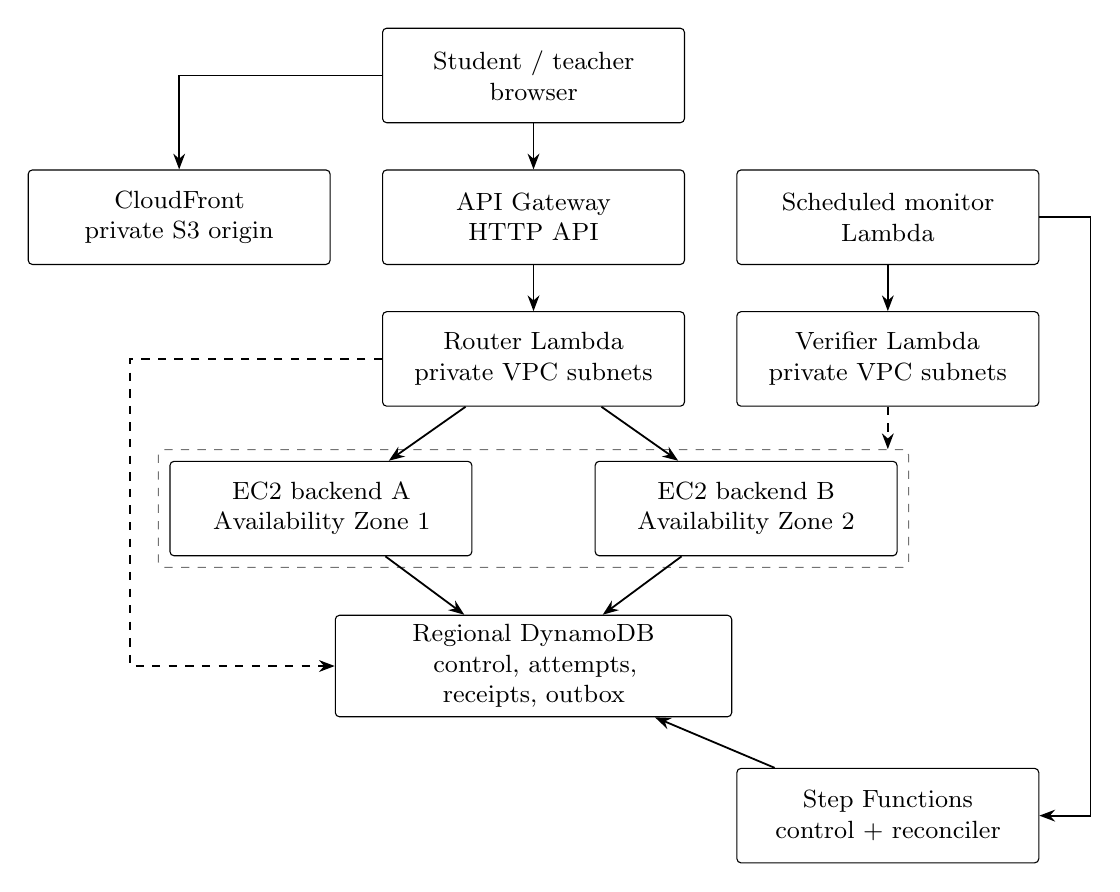
\begin{tikzpicture}[node distance=8mm and 12mm]
\node[box] (browser) at (0,0) {Student / teacher\\browser};
\node[box] (static) at (-4.5,-1.8) {CloudFront\\private S3 origin};
\node[box] (api) at (0,-1.8) {API Gateway\\HTTP API};
\node[box] (router) at (0,-3.6) {Router Lambda\\private VPC subnets};
\node[box] (a) at (-2.7,-5.5) {EC2 backend A\\Availability Zone 1};
\node[box] (b) at (2.7,-5.5) {EC2 backend B\\Availability Zone 2};
\node[group,fit=(a)(b),inner sep=4pt] (tier) {};
\node[box,text width=48mm] (ddb) at (0,-7.5) {Regional DynamoDB\\control, attempts, receipts, outbox};
\node[box] (monitor) at (4.5,-1.8) {Scheduled monitor\\Lambda};
\node[box] (verifier) at (4.5,-3.6) {Verifier Lambda\\private VPC subnets};
\node[box] (workflow) at (4.5,-9.4) {Step Functions\\control + reconciler};
\draw[arrow] (browser)--(api);
\draw[arrow] (browser)-|(static);
\draw[arrow] (api)--(router);
\draw[arrow] (router)--(a);
\draw[arrow] (router)--(b);
\draw[arrow] (a)--(ddb);
\draw[arrow] (b)--(ddb);
\draw[arrow] (monitor)--(verifier);
\draw[arrow,dashed] (verifier.south)--(verifier.south |- tier.north);
\draw[arrow] (monitor.east)--++(.65,0)|-(workflow.east);
\draw[arrow] (workflow)--(ddb);
\draw[arrow,dashed] (router.west)--++(-3.2,0)|-(ddb.west);
\end{tikzpicture}
\caption[Logical cloud architecture and regional recovery services]{Logical cloud architecture. Regional services run in Sydney; CloudFront provides global content delivery. Dashed paths show the router's control-record read and the verifier's probes of the grouped A/B tier.}\label{fig:cloud}
\end{figure}

\FloatBarrier
\section{Application and Routing Components}
The two EC2 instances run the Go application with a shared regional store. They are assigned identities A and B. A strongly consistent read of the active control record provides the router with the current backend and epoch. The router supplies those values as internal request metadata when it forwards a request over the private application address.

The record is stored at partition key \texttt{CONTROL\#ACTIVE} and sort key \texttt{STATE}. Its important fields are \texttt{active\_backend}, \texttt{epoch}, and \texttt{paused}. An epoch identifies a particular grant of writer authority, rather than simply identifying a machine. Returning authority to A after a recovery must therefore use a newer epoch than A held previously.

There are two layers of protection. Request middleware propagates writer context into application operations, and storage transactions validate that context against the current control record. The second layer is essential: a route can change between the router's read and the backend's database write.
\section{Network Design}
The VPC contains application and Lambda subnets across two Availability Zones. Application instances use public subnets and automatic public IPv4 addresses for bootstrap and Systems Manager connectivity. Their application port is nevertheless private in use: inbound TCP port 8000 is allowed only from the router/verifier security group, and no inbound SSH rule is created.

The router and verifier use private Lambda subnets. S3 and DynamoDB gateway endpoints are associated with the relevant route tables. No NAT gateway is provisioned. Functions that call public AWS APIs or perform the public smoke test remain outside the application VPC. Connecting a Lambda function to a public subnet would not itself provide internet access~\cite{aws-lambda-vpc}; the architecture instead assigns functions according to their actual network dependencies.


\begin{table}[!htbp]\centering\small
\caption{Component placement and responsibility}\label{tab:placement}
\begin{tabularx}{\textwidth}{@{}L{33mm}L{42mm}Y@{}}\toprule
\textbf{Component} & \textbf{Placement} & \textbf{Responsibility}\\\midrule
Frontend & S3 and CloudFront & Static application delivery\\
Router & Private VPC Lambda subnets & Authoritative route read and HTTP forwarding\\
Verifier & Private VPC Lambda subnets & Probe A/B and apply protected fault controls\\
Application A/B & Separate EC2 Availability Zones & Assessment and classroom HTTP operations\\
Monitor & Lambda outside the VPC & Repeated incident confirmation and workflow start\\
Control & Lambda outside the VPC & Lease, promotion, public smoke, instance controls\\
Reconciler & Lambda outside the VPC & Bounded outbox processing\\
Data store & Regional DynamoDB & Shared durable application and control state\\\bottomrule
\end{tabularx}\end{table}

\section{Liveness and Application Readiness}
Liveness answers whether the process responds. Deep readiness answers whether it can currently serve the assessment path under the configured checks. The probe calls \texttt{/health/live} and \texttt{/health/deep} separately with bounded timeouts. Deep health includes database capability and configured host/application checks.

The partial-failure scenario injects a database-access stall into one application. Its process remains alive, but readiness becomes false. This tests a useful distinction without claiming that the DynamoDB service itself failed. When both backends fail readiness, the monitor suppresses promotion because switching to the standby would not establish a usable target.

\begin{table}[!htbp]\centering\small
\caption{Readiness decision policy for the active and standby backends}\label{tab:health-decisions}
\begin{tabularx}{\textwidth}{@{}L{27mm}L{28mm}Y@{}}\toprule
\textbf{Active ready} & \textbf{Standby ready} & \textbf{Recovery decision}\\\midrule
Yes & Yes & Keep the current writer; no failure is established\\
Yes & No & Keep the current writer and restore standby capability\\
No & Yes & Confirm sustained failure, acquire the lease, and recheck before promotion\\
No & No & Suppress promotion; a usable target has not been established\\\bottomrule
\end{tabularx}\end{table}

Readiness observations are evidence for a decision, not permanent guarantees. The candidate is checked again while the incident lease is held because its condition may change after the monitor's last observation. Liveness remains useful for distinguishing a stopped HTTP server from a responding process with a failed dependency.
\section{Confirmation Policy}
The cloud monitor is triggered by an EventBridge scheduled rule once per minute. Within a monitor invocation, the policy requires three observations separated by five seconds. These observations must refer to the same active backend and epoch. A route change, a paused control plane, recovered active readiness, or an unhealthy standby prevents automatic promotion.

Three samples contain two configured waiting intervals, giving ten seconds of deliberate spacing before probe and invocation overhead. The schedule can also introduce delay before the first sample. Consequently, the policy does not imply a ten-second fault-to-recovery guarantee.
\section{Recovery Workflow}
After confirmation, the Standard workflow acquires an incident lease and performs a fresh verification under that lease. The conditional promotion checks the expected backend, expected epoch, live lease ownership, and unpaused state. The target backend receives the next epoch.


\begin{figure}[htbp]\centering
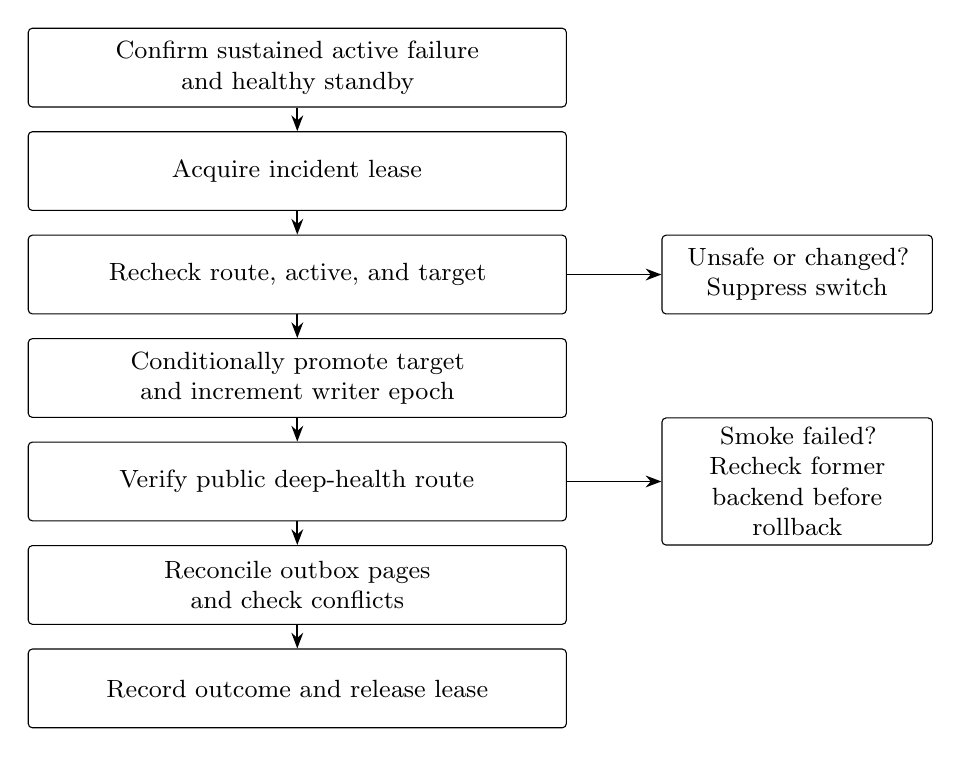
\begin{tikzpicture}[node distance=3mm,box/.append style={minimum height=10mm}]
\node[box,text width=66mm] (confirm) {Confirm sustained active failure\\and healthy standby};
\node[box,text width=66mm,below=of confirm] (lease) {Acquire incident lease};
\node[box,text width=66mm,below=of lease] (verify) {Recheck route, active, and target};
\node[box,text width=66mm,below=of verify] (promote) {Conditionally promote target\\and increment writer epoch};
\node[box,text width=66mm,below=of promote] (smoke) {Verify public deep-health route};
\node[box,text width=66mm,below=of smoke] (reconcile) {Reconcile outbox pages\\and check conflicts};
\node[box,text width=66mm,below=of reconcile] (done) {Record outcome and release lease};
\node[box,text width=32mm,right=12mm of verify] (suppress) {Unsafe or changed?\\Suppress switch};
\node[box,text width=32mm,right=12mm of smoke] (rollback) {Smoke failed?\\Recheck former\\backend before\\rollback};
\draw[arrow] (confirm)--(lease);\draw[arrow] (lease)--(verify);
\draw[arrow] (verify)--(promote);\draw[arrow] (promote)--(smoke);
\draw[arrow] (smoke)--(reconcile);\draw[arrow] (reconcile)--(done);
\draw[arrow] (verify)--(suppress);\draw[arrow] (smoke)--(rollback);
\end{tikzpicture}
\caption[Verified recovery sequence and safety branches]{Recovery sequence and the principal safety branches. The workflow records a successful outcome only after the required verification and reconciliation checks.}\label{fig:workflow}
\end{figure}

\FloatBarrier
The public smoke test traverses the externally reachable API and checks deep health through the selected route. A failed smoke result cannot be converted into a successful recovery. Rollback requires fresh readiness of the former backend and advances the epoch again; the controller cannot safely restore an old authority value.

Reconciliation is a separate phase. It scans pending journal work in bounded pages, verifies canonical submission records, and records completion only after the required checks succeed. Manual reconciliation also runs asynchronously through a workflow, so the public action request does not wait for the full backlog.

Lease ownership uses explicit expiry timestamps in conditional operations, independent of asynchronous DynamoDB TTL cleanup. Error paths release the lease; expiry bounds ownership if execution stops.

\chapter{Data Design and Correctness Mechanisms}
\section{Logical Data Model}
Continuum uses a single DynamoDB table with partition and sort keys to represent distinct entity types. The application store manages users, classroom membership, assessment metadata, attempts, submissions, receipts, and outbox entries. Control and audit namespaces support the recovery machinery.


\begin{table}[htbp]\centering\small
\caption{Principal logical records in the assessment recovery path}\label{tab:records}
\begin{tabularx}{\textwidth}{@{}L{28mm}YY@{}}\toprule
\textbf{Record} & \textbf{Important information} & \textbf{Purpose}\\\midrule
Active control & Backend, epoch, paused state & Authoritative route and writer identity\\
Incident lease & Owner and explicit expiry & Serialise recovery ownership\\
Assessment & Questions, duration, windows, policy & Define delivery and grading rules\\
Attempt & Learner, answers, start, version, attempt number & Resume work and enforce lifecycle\\
Submission & Immutable attempt snapshot and latest reference & Retain the accepted answer outcome\\
Request receipt & Request ID, payload hash, scope, commit time & Resolve exact retries\\
Outbox journal & Target submission, request ID, processed flag & Recover interrupted audit processing\\
Audit summary & Request ID and canonical target reference & Record one validated downstream outcome\\\bottomrule
\end{tabularx}\end{table}

The current implementation supports attempt-scoped submission history and a latest-submission reference. The recorded October cloud rehearsal predates some broader product additions; its counts refer to the canonical submission and recovery records inspected for that particular request. Logical submission counts should not be confused with the number of physical records used by a newer schema.
\section{Writer Epoch and Atomic Fencing}
Let the authoritative control state be
\begin{equation}
C=(b,e,p),
\end{equation}
where $b$ is the active backend, $e$ is its epoch, and $p$ is the paused flag. A request carries the writer identity $W=(b_w,e_w)$. A protected mutation is permitted only if
\begin{equation}\label{eq:fence}
b_w=b\quad\land\quad e_w=e\quad\land\quad p=\mathrm{false}.
\end{equation}
The database evaluates this condition in the same \texttt{TransactWriteItems} operation as the application changes. A preliminary read alone would be insufficient, because a promotion could occur between that read and the commit.

Consider a request routed to A at epoch 1. If promotion commits B at epoch 2 before the request's write transaction, condition~\eqref{eq:fence} fails for A. If A's transaction commits first, its data belongs to the preceding valid writer interval. This establishes an ordering at the storage boundary. It does not require the failed process to receive a notification or stop immediately.

Failback and rollback obey the same rule. Returning to A after B does not reuse epoch 1; it advances to a newer epoch. An old request therefore cannot become valid again merely because its original backend name is active once more.

\subsection{The Race Between a Submission and Promotion}
The decisive event is the database commit order. Table~\ref{tab:race-order} considers a request already executing on A at epoch 1 while the controller attempts to promote B. A routing header identifies the proposed writer; it is not by itself proof of continuing authority.
\begin{table}[htbp]\centering\small
\caption{Ordering of an in-flight write and a conditional promotion}\label{tab:race-order}
\begin{tabularx}{\textwidth}{@{}L{43mm}YY@{}}\toprule
\textbf{Ordering} & \textbf{Storage outcome} & \textbf{Client implication}\\\midrule
A/1 transaction commits first & A's records belong to a valid epoch-1 writer interval & A lost response can be resolved from the durable receipt\\
B/2 promotion commits first & A/1 fails the writer condition; the protected transaction does not commit & Retry through the current route using the retained request identity\\
Promotion response is lost & A retry is checked against the same lease and expected next epoch & Repeated control work must not advance authority twice for one operation\\
A later becomes active again & A receives a newer epoch & An old A/1 request remains invalid\\\bottomrule
\end{tabularx}\end{table}

The guarantee concerns protected writes using the shared control condition. It does not turn every application read into a global serialisable snapshot, and it does not recover a regionally unavailable data store.
\section{Request Identity and Payload Binding}
Each final submission has a persistent request identifier $r$. The browser retains the identifier together with the immutable answer snapshot being submitted. The server binds that request to its assessment, learner, attempt, and payload through a deterministic hash. Conceptually,
\begin{equation}
K_r=(r,\text{assessment},\text{learner},\text{attempt},H(a)).
\end{equation}
A retry of the same logical request retrieves the original receipt. Reusing $r$ with changed answers or a mismatched scope is a conflict. This prevents a response-lost retry from silently becoming a different answer submission.

The application receipt is stored durably and contains the committed timestamp, request identifier, version, score, total, and attempt number. Its lifetime and lookup semantics belong to the application data model. They are distinct from a temporary database-client request token.
\section{Atomic Submission Transaction}
The current store builds the final submission using one transaction containing the following writes and condition:
\begin{enumerate}
\item Create the immutable submission snapshot for the attempt.
\item Update the latest-submission reference.
\item Create the request receipt if that request has not already committed.
\item Create the pending outbox journal entry.
\item Mark the active attempt submitted using version and attempt-number conditions.
\item Check the authoritative backend, epoch, and unpaused state.
\end{enumerate}
The attempt condition prevents an outdated version from completing a conflicting lifecycle transition. The uniqueness conditions prevent duplicate receipt and snapshot creation. Atomicity ensures that the application does not acknowledge a final submission without its corresponding receipt and recovery journal.


\begin{figure}[htbp]\centering
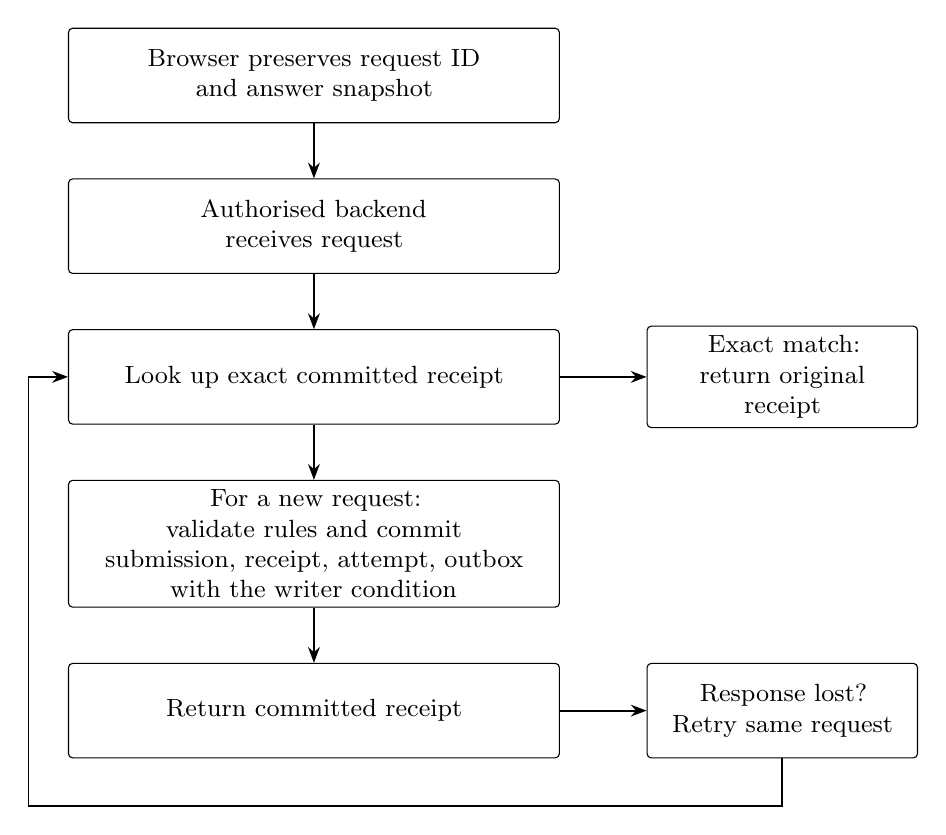
\begin{tikzpicture}[node distance=7mm]
\node[box,text width=60mm] (client) {Browser preserves request ID\\and answer snapshot};
\node[box,text width=60mm,below=of client] (api) {Authorised backend\\receives request};
\node[box,text width=60mm,below=of api] (lookup) {Look up exact committed receipt};
\node[box,text width=60mm,below=of lookup] (transaction) {For a new request:\\validate rules and commit\\submission, receipt, attempt, outbox\\with the writer condition};
\node[box,text width=60mm,below=of transaction] (response) {Return committed receipt};
\node[box,text width=32mm,right=11mm of lookup] (duplicate) {Exact match:\\return original\\receipt};
\node[box,text width=32mm,right=11mm of response] (retry) {Response lost?\\Retry same request};
\draw[arrow] (client)--(api);\draw[arrow] (api)--(lookup);
\draw[arrow] (lookup)--(transaction);\draw[arrow] (transaction)--(response);
\draw[arrow] (lookup)--(duplicate);\draw[arrow] (response)--(retry);
\draw[arrow] (retry.south)--++(0,-.6)-|($(lookup.west)+(-.5,0)$)--(lookup.west);
\end{tikzpicture}
\caption[Submission and exact receipt replay contract]{Submission and receipt replay contract. An exact retry follows the lookup path; a changed payload under the original identifier is rejected.}\label{fig:receipt-flow}
\end{figure}

\FloatBarrier
\section{Attempt Timing and Receipt Replay}
\label{sec:timing-policy}
The server persists the attempt start time. In the current store, the effective attempt deadline is recalculated from that start and the current assessment duration:
\begin{equation}
D_{\mathrm{attempt}}=t_{\mathrm{start}}+60\,000\,d_{\mathrm{current}},
\end{equation}
where timestamps are in milliseconds and duration $d$ is in minutes. A backend change does not recreate the attempt, so the deadline remains the same when the assessment metadata is unchanged. The fresh demonstration assessment has a 15-minute duration and one attempt.

This is a narrower property than freezing assessment policy at attempt creation. Changing the duration while an attempt is running changes the calculated deadline. Availability-window checks and late-work settings are also evaluated separately. The service checks the attempt deadline before calling the store, with a default five-second grace period; the write transaction checks the attempt version and writer authority, but does not independently compare commit time with a frozen deadline. These details define the current timing semantics and motivate policy snapshots and commit-boundary tests for institutional deployment.

For a new submission, the service enforces the configured rules and its bounded server-side grace policy. An exact committed receipt is looked up before rejecting the request because the exam has since closed. Retrieving proof of a previous commit does not constitute accepting new answers after the deadline. If no matching receipt exists, ordinary deadline checks still apply.

The browser presents local buffering separately from confirmed storage. An answer retained on the student's device is useful for retry, but it cannot establish that the server accepted the final submission. A prolonged outage may outlast the student's remaining permitted time; the architecture does not promise recovery of every uncommitted offline answer.
\section{Transactional Outbox and Audit Reconciliation}
An outbox entry is created atomically with the submission. It describes pending downstream work and points to the canonical submission. The reconciler reads pending entries, checks that the target and request identity agree, and creates an answer-free audit summary while marking the journal processed.

These operations are conditional and atomic. Repeated reconciliation therefore does not add another logical audit outcome for the same request. A matching pre-existing audit can repair a pending journal only after the canonical target and complete key are checked. Conflicts are reported rather than overwritten.

The journal may carry answer information needed by the implementation; the resulting audit summary omits the answers. This distinction matters for access control and retention. The reconciler is not a general-purpose message broker or a proof of exactly-once processing for arbitrary external systems.

\subsection{Interruption Points and Recovery}
If execution stops before the submission transaction commits, there is no accepted final outcome from that transaction. If it stops after commit but before returning a response, the receipt is already present. If it stops before audit reconciliation, the pending journal remains discoverable. If reconciliation is retried after completion, its conditions identify the existing logical result.

This design removes the unsafe gap in which a submission could commit without the journal describing its required audit work. It also prevents a secondary audit step from becoming part of the learner's synchronous request latency. The trade-off is that reconciliation must scan or otherwise locate pending work, monitor conflicts, and retain records long enough to repair interruptions.

These properties depend on every protected mutation using the writer condition, exact replay retaining its payload-bound receipt, and the regional store remaining available. They establish a bounded assessment contract rather than exactly-once behaviour for arbitrary external systems.

\chapter{Implementation and Application Workflows}
\section{From Architecture to a Working Assessment}
The recovery mechanism is integrated with an application that teachers and learners can use. A teacher prepares and publishes a classroom assessment; a learner enters it, answers against a server-managed attempt, and receives a submission reference. These operations exercise authentication, authorisation, persistence, grading, and recovery through the same public API.

The screens in this chapter were captured from the running application on 23 October 2026 using a synthetic BCSE355L classroom and a five-question, fifteen-minute assessment~\cite{local-capture}. They show local mode: two backend HTTP servers share an in-memory store within one process. They establish the implemented user workflow; the separate AWS experiment in Chapter~6 supplies evidence for cloud recovery.

\begin{figure}[H]\centering
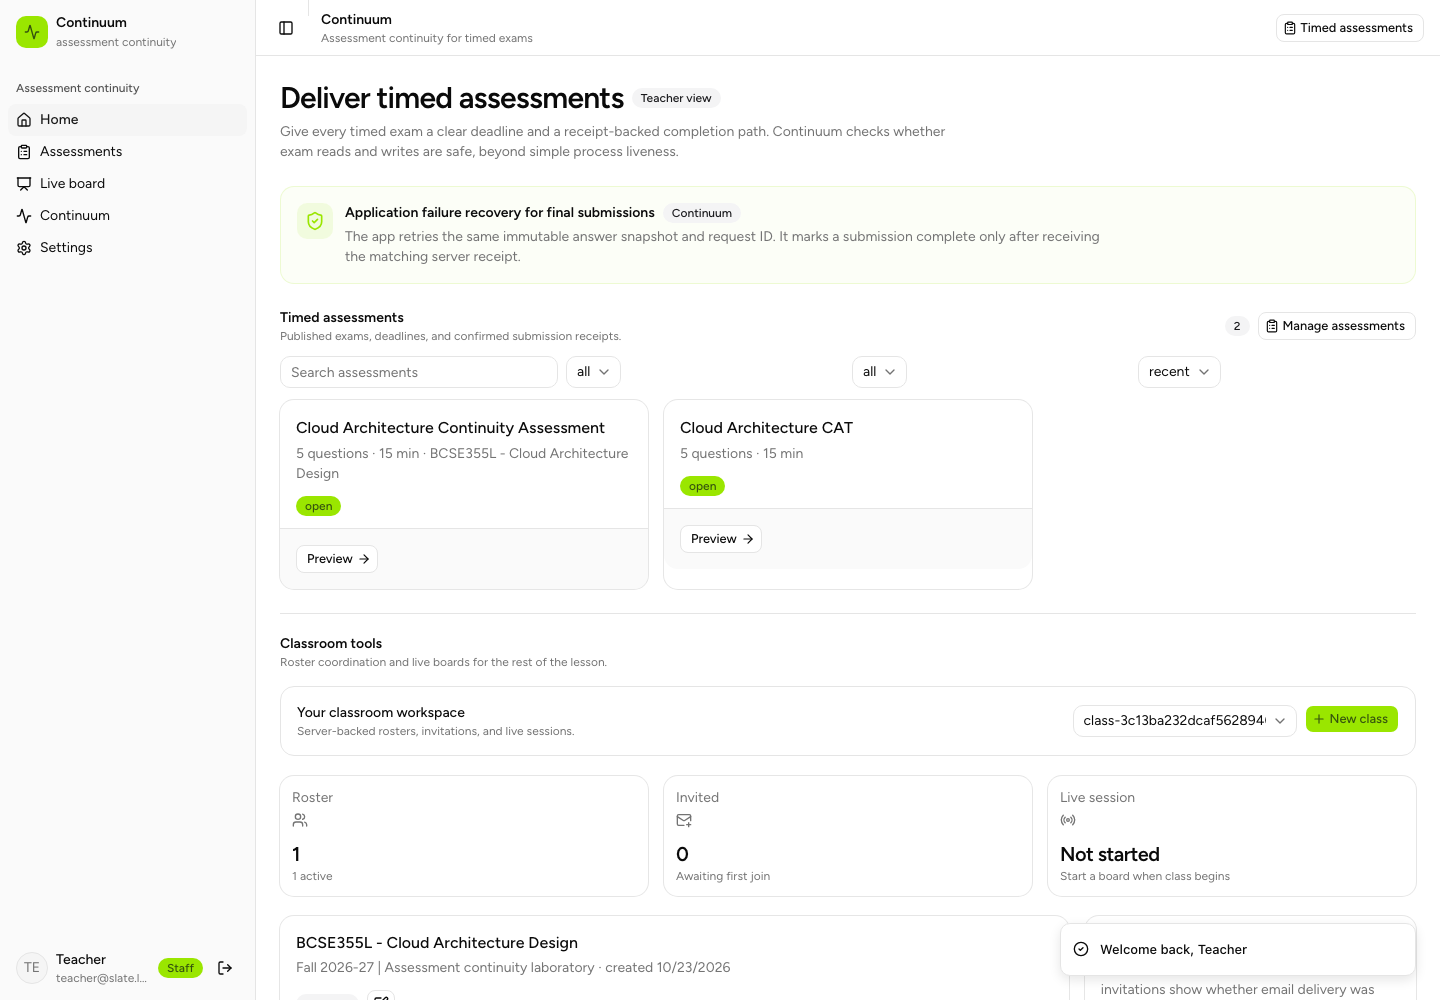
\includegraphics[width=\textwidth,trim=265bp 230bp 15bp 60bp,clip]{screenshots/teacher-dashboard.png}
\caption[Teacher home and classroom overview]{Teacher home with classroom context and assessment actions, using synthetic course data.}\label{fig:teacher-home}
\end{figure}

\Needspace{10\baselineskip}
\section{Teacher Preparation and Publication}
The editor captures the title, classroom, instructions, duration, and attempt limit. Each question has options, a correct choice, points, and feedback. The example uses five two-point questions, making the maximum score ten.

A draft permits preparation before learners see the assessment. Publishing exposes it through the catalogue. Published questions are protected against changes to an existing grading basis; availability and instructions remain separately managed~\cite{project-source}.

Classroom membership and API role checks protect assessment access and management. Retakes create a new attempt context while preserving earlier receipts.

\begin{figure}[H]\centering
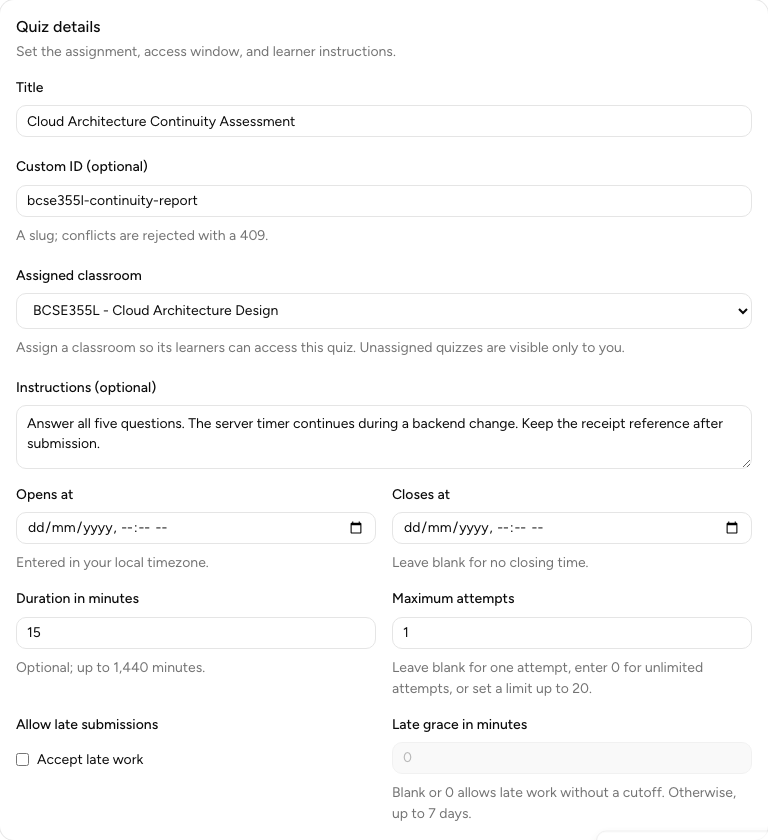
\includegraphics[width=125mm]{screenshots/teacher-assessment-settings.png}
\caption[Assessment policy settings]{Assessment policy: classroom assignment, instructions, a fifteen-minute duration, and one allowed attempt.}\label{fig:teacher-policy}
\end{figure}

\begin{figure}[H]\centering
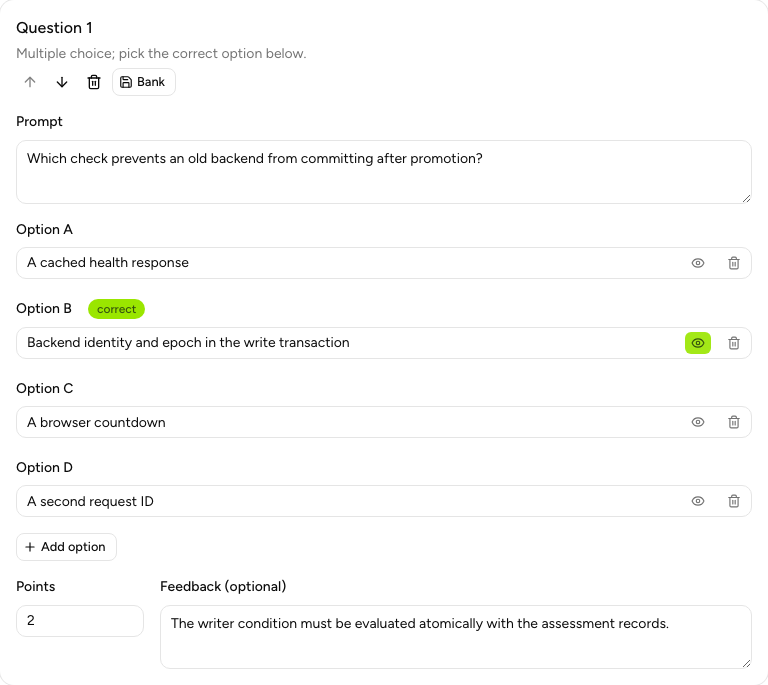
\includegraphics[width=125mm]{screenshots/teacher-question-editor.png}
\caption[Question authoring and grading configuration]{Question authoring with a selected correct option, explicit points, and explanatory feedback.}\label{fig:question-editor}
\end{figure}

\begin{figure}[H]\centering
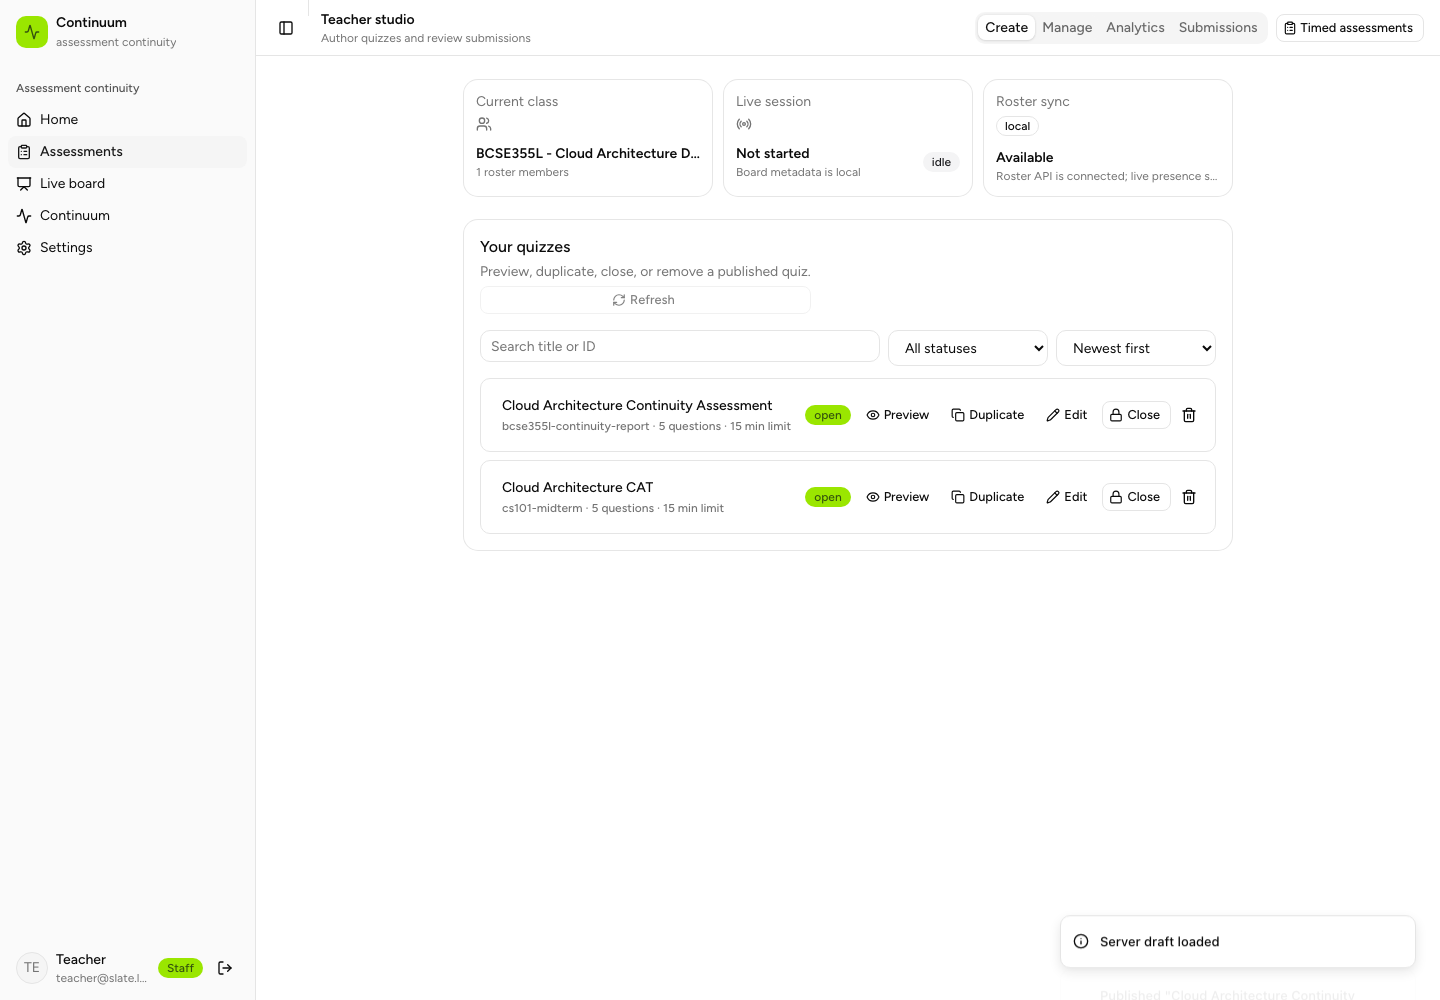
\includegraphics[width=150mm,trim=430bp 430bp 140bp 65bp,clip]{screenshots/teacher-published-assessment.png}
\caption[Published assessment management]{Teacher management view after publication, with availability and lifecycle controls.}\label{fig:published}
\end{figure}

\FloatBarrier
\section{Learner Entry and Timed Answering}
After authentication, the learner sees assessments permitted by classroom membership. The catalogue supports discovery; the lobby explains the selected assessment before the learner starts. Starting obtains the server-managed attempt and its persisted start time. Changing backend does not create another start event.

\begin{figure}[H]\centering
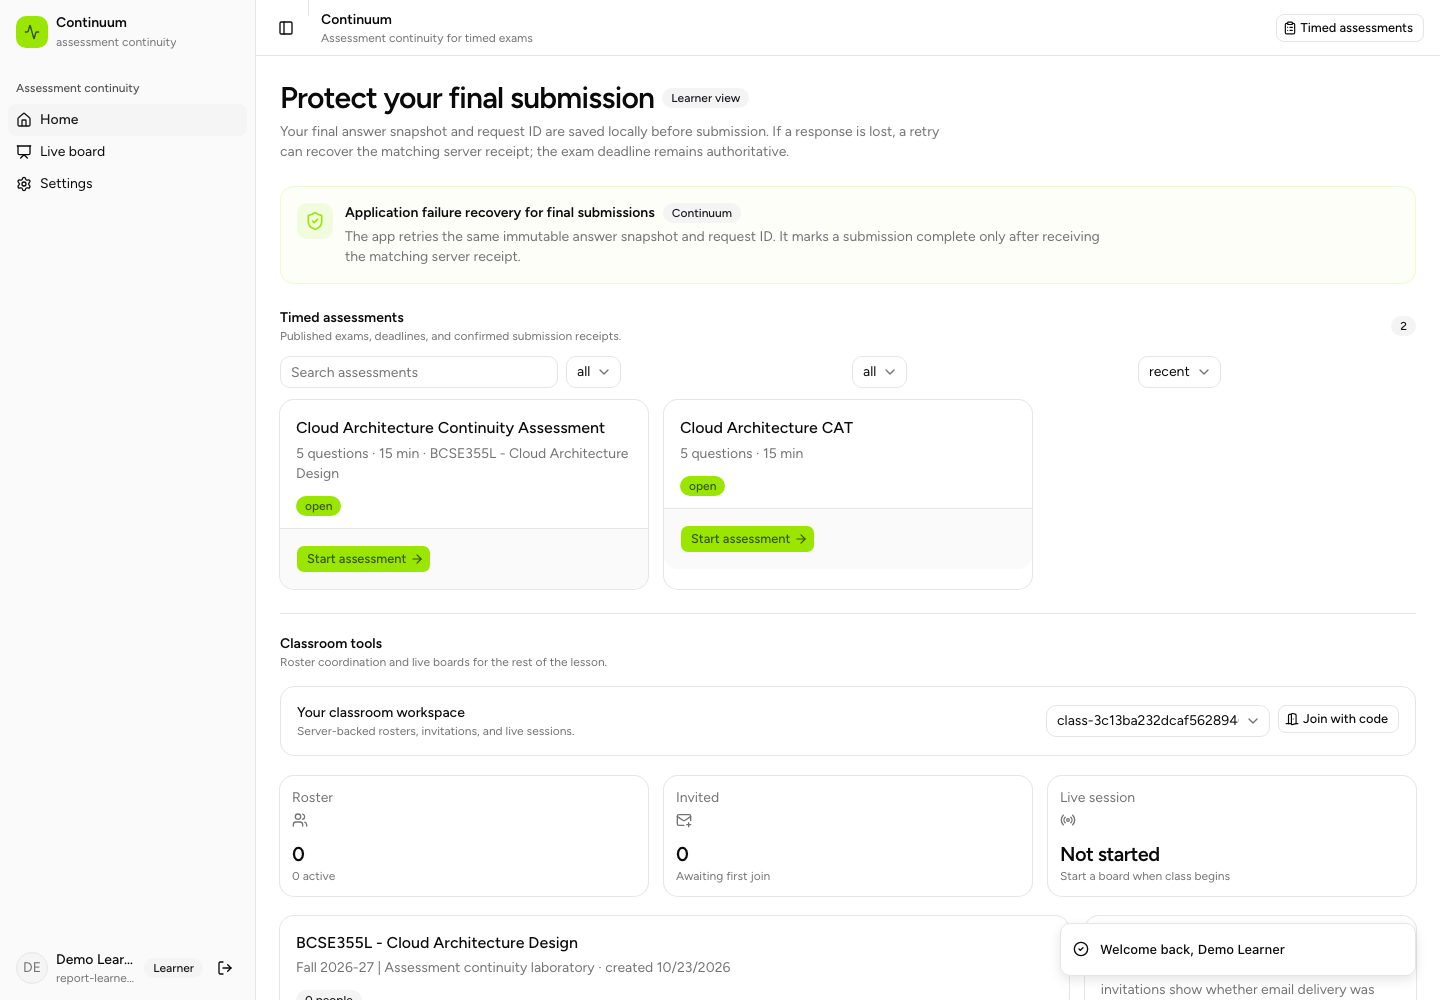
\includegraphics[width=\textwidth,trim=265bp 390bp 15bp 60bp,clip]{screenshots/learner-assessment-catalog.png}
\caption[Learner assessment catalogue]{Learner catalogue containing the published Cloud Architecture Continuity Assessment.}\label{fig:catalogue}
\end{figure}

\begin{figure}[H]\centering
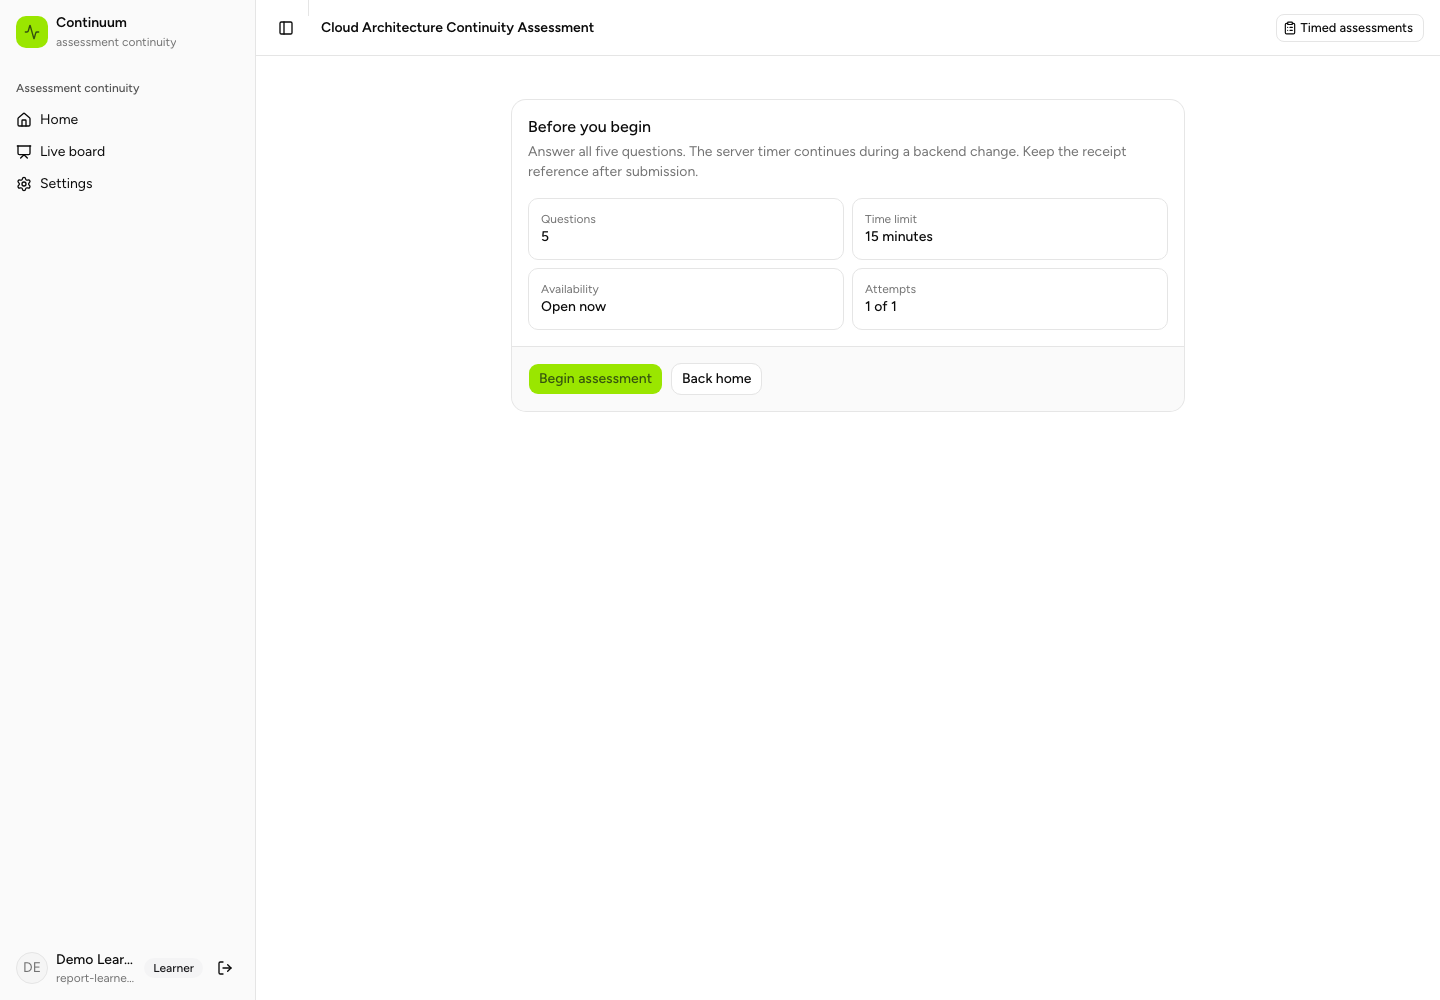
\includegraphics[width=\textwidth,trim=480bp 560bp 220bp 85bp,clip]{screenshots/learner-assessment-lobby.png}
\caption[Assessment lobby and start policy]{Assessment lobby showing instructions and the policy before the timed attempt begins.}\label{fig:lobby}
\end{figure}

\Needspace{5\baselineskip}
Within the assessment, navigation separates answering from review. A learner can select an answer, flag a question, revisit unanswered questions, and inspect the remaining time before submission. These controls help the learner identify what remains to be done without creating a second attempt during an interruption.

\begin{figure}[H]\centering
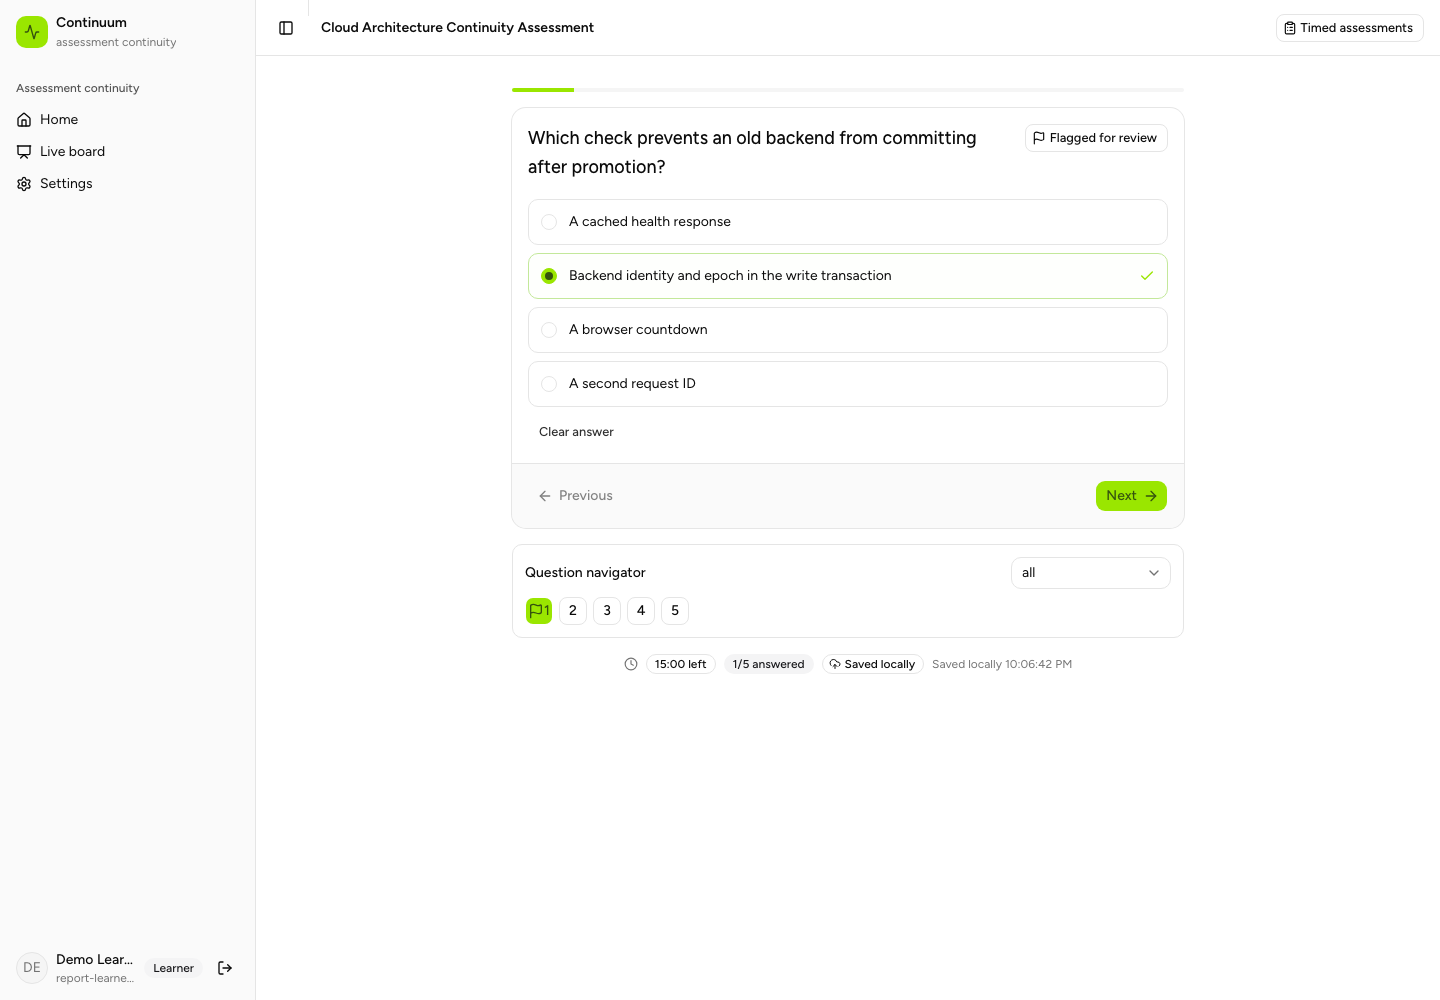
\includegraphics[width=\textwidth,trim=480bp 300bp 220bp 75bp,clip]{screenshots/learner-answer-and-review.png}
\caption[Timed answering and review controls]{Timed answering with a selected choice, review flag, question navigation, remaining time, and local-save status.}\label{fig:answer-review}
\end{figure}

\subsection{Three Different Meanings of Saved}
Browser storage, acknowledged progress, and a committed final result are separate states. ``Saved locally'' means this browser retained progress; a successful save response acknowledges backend attempt state. Only a final receipt identifies the immutable submitted snapshot and committed outcome.

Figure~\ref{fig:resume} demonstrates continuation from device state, rather than durability after browser loss. Backend changes preserve the attempt start time. Its deadline also depends on the current duration setting; Section~\ref{sec:timing-policy} explains that policy boundary.

\begin{figure}[H]\centering
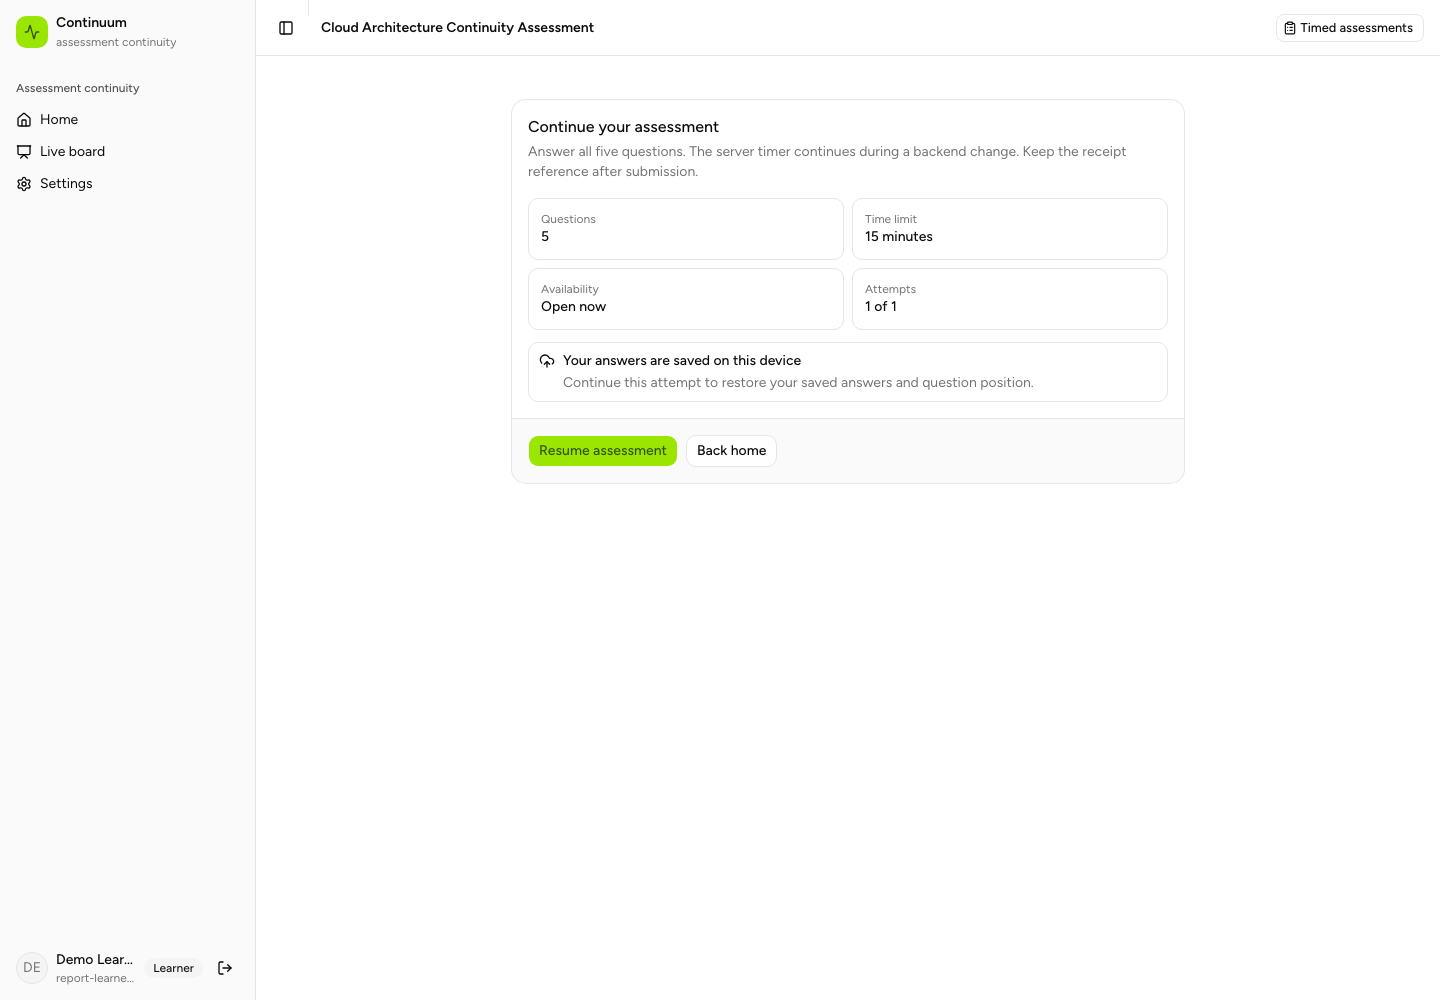
\includegraphics[width=150mm,trim=480bp 500bp 220bp 85bp,clip]{screenshots/learner-resume-attempt.png}
\caption[Continuing a saved attempt]{Continuation prompt after revisiting the assessment. The interface identifies answers retained on this device.}\label{fig:resume}
\end{figure}

\FloatBarrier
\section{Final Submission and Receipt Retrieval}
Before final submission, the browser preserves a request identifier with a fixed answer snapshot. Bounded retries use this identity rather than generating a different logical submission for every network attempt. A transport error may leave the outcome unknown, so the interface resolves the receipt before asking the learner to create a new submission.

Figure~\ref{fig:local-receipt} shows the completed synthetic attempt: score, submission time, receipt reference, copy/download actions, and question feedback. This local capture illustrates receipt retrieval through the application. It is not the response-loss experiment; equality of the original and replayed AWS commit is established independently in Chapter~6.

\begin{figure}[!htbp]\centering
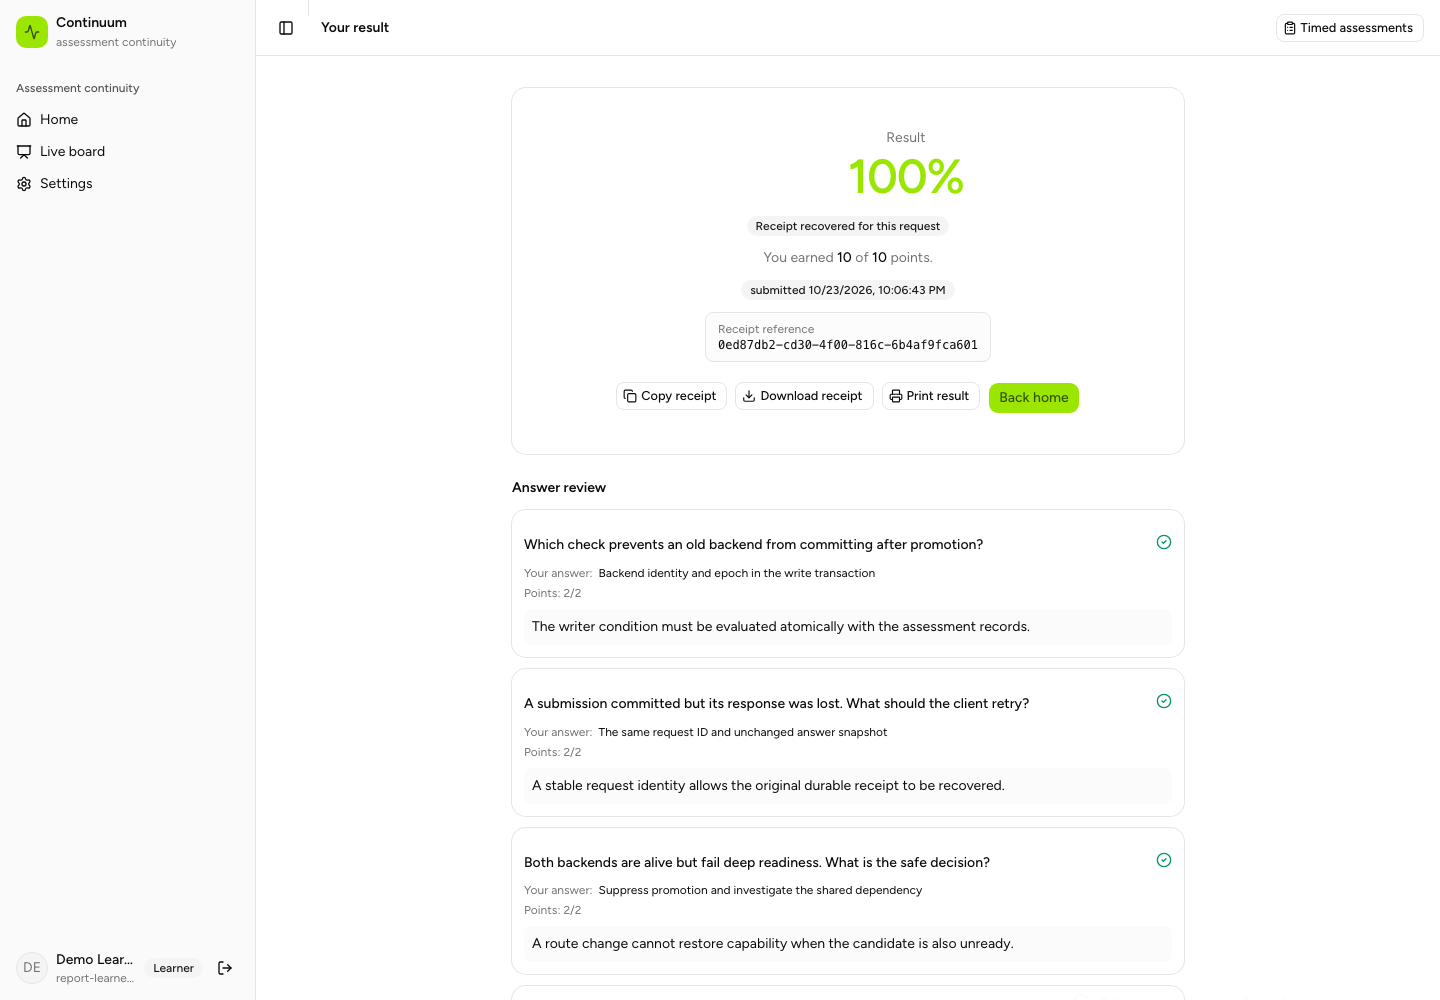
\includegraphics[width=150mm,trim=480bp 320bp 220bp 75bp,clip]{screenshots/learner-committed-receipt.png}
\caption[Retrieved local submission receipt and feedback]{Retrieved local result with a receipt reference, submission time, and answer review. The synthetic learner earned ten of ten points.}\label{fig:local-receipt}
\end{figure}

\section{Code Structure and Deployment}
Go implements the backend; React and TypeScript implement the interface. TanStack Router and Query coordinate navigation and server state, while Vite and Tailwind CSS support the frontend build. The AWS implementation uses the Go SDK v2 and Terraform. Table~\ref{tab:modules} identifies the boundaries that make the recovery contract reviewable.

\begin{table}[htbp]\centering\small
\caption{Implementation boundaries and the contracts they protect}\label{tab:modules}
\begin{tabularx}{\textwidth}{@{}L{53mm}Y@{}}\toprule
\textbf{Source boundary} & \textbf{Responsibility}\\\midrule
\path{internal/httpapi} & Authentication, classroom access, validation, and response mapping\\
\path{internal/exams} & Availability, attempt timing, saving, retakes, and submission rules\\
\path{internal/store} & Memory/DynamoDB persistence; receipts, attempts, transactional writes\\
\path{internal/clusterstate} & Authoritative backend/epoch contract for protected writes\\
\path{internal/continuum} & Router, capability probes, monitoring, control state, and events\\
\path{cmd/demo-reconciler} & Conditional outbox processing and audit completion\\
\path{statemachine/demo-failover.asl.json} & Recovery sequence, verification, and error paths\\
\path{infra/demo} & Supported single-Region AWS deployment\\
\path{web/src} & Role workflows, pending requests, and receipt presentation\\\bottomrule
\end{tabularx}\end{table}

Build scripts package application and Lambda artifacts deterministically. Bootstrap retrieves a private bundle and encrypted runtime configuration. A full deployment can replace instances and therefore requires a maintenance window. Pause/resume preserves the desired instance and monitoring state; private deployment files remain outside the report package.

\chapter{Experimental Evaluation and Discussion}
\section{Questions and Evidence}
The evaluation asks four questions: does recovery restore a usable public route; can the learner resolve a submission whose response was lost; does an obsolete backend lose write authority; and does repeated reconciliation avoid another logical audit result? Each requires different evidence. A green health indicator answers only the first; request comparison and database inspection are needed for the second and fourth.

The evidence comprises current-source backend checks, fresh local interface and fault captures on 23 October 2026, and the preserved AWS rehearsal of 10 October 2026. Local mode verifies behaviour through real HTTP servers, but its shared process and memory store do not reproduce EC2 isolation or DynamoDB durability. AWS observations apply to the recorded deployment and synthetic workload~\cite{project-source,local-capture,cloud-run,cloud-records}.

\begin{table}[H]\centering\small
\caption{Evidence layers and their limits}\label{tab:evidence-layers}
\begin{tabularx}{\textwidth}{@{}L{30mm}YY@{}}\toprule
\textbf{Layer} & \textbf{Useful evidence} & \textbf{Important limit}\\\midrule
Source and tests & Conditions, timing rules, race cases, replay and conflicts & Cannot establish a deployed cloud outcome alone\\
Local application & Role workflows, probe decisions, HTTP recovery, receipt display & Shared process and non-durable memory\\
AWS rehearsal & Actual instance stop, promoted route, replay, record inspection & One bounded run, not a latency distribution\\\bottomrule
\end{tabularx}\end{table}

\section{Backend Verification}
On 23 October 2026, six existing Go package suites passed with the race detector enabled. This package-level result does not imply that every production workload or fault ordering has been tested. Appendix~A retains the commands.

\begin{table}[H]\centering\small
\caption{Current-source backend verification}\label{tab:verification}
\begin{tabularx}{\textwidth}{@{}L{53mm}Y L{16mm}@{}}\toprule
\textbf{Package} & \textbf{Coverage focus} & \textbf{Result}\\\midrule
\path{internal/continuum} & Routing, promotion, leases, readiness, events & Passed\\
\path{internal/store} & Writer conditions, receipts, attempts, durable entities & Passed\\
\path{cmd/demo-reconciler} & Reconciliation and conflict handling & Passed\\
\path{integration} & Real HTTP response loss, recovery, exact replay & Passed\\
\path{internal/httpapi} & Validation, access, lifecycle, receipts & Passed\\
\path{internal/exams} & Assessment rules, timing, attempts & Passed\\\bottomrule
\end{tabularx}\end{table}

The preserved implementation review separately records frontend checks, production builds, Terraform validation, and state-machine validation~\cite{project-review}. Those historical results complement the backend suites; they were not additional checks rerun during screenshot capture.

\section{Local Fault Decisions}
The first local sequence disabled application readiness on both backends while their liveness probes still passed. The screen retained A at epoch 1 and recorded suppression (Figure~\ref{fig:unsafe}). This is the intended response: routing to another unready process cannot restore the operation the learner needs.

\begin{figure}[htbp]\centering
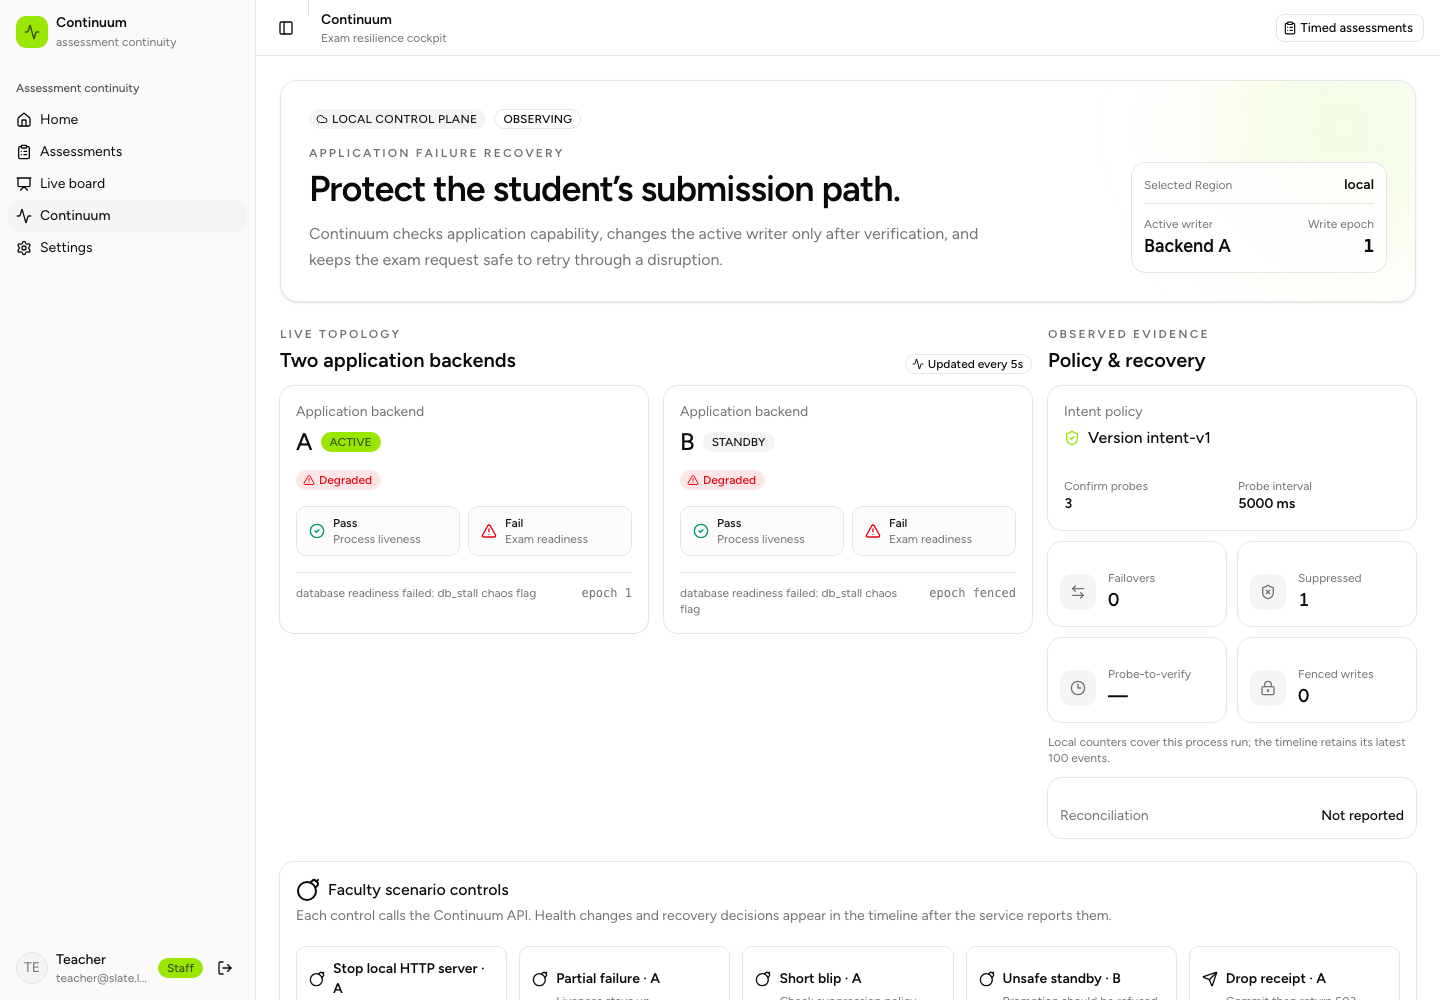
\includegraphics[width=\textwidth,trim=270bp 155bp 15bp 75bp,clip]{screenshots/recovery-unsafe-standby.png}
\caption[Local suppression when both backends are unready]{Local unsafe-standby case: both processes are alive but fail assessment readiness. Promotion is suppressed and A retains epoch 1.}\label{fig:unsafe}
\end{figure}

After clearing the faults, the active A HTTP server was stopped. Three consecutive failed probes led to B becoming active at epoch 2. The local screen reports 10,010\,ms from the first failed monitor probe to route verification. This excludes the earlier wait for that first probe and is separate from the AWS recovery measurement.

\begin{figure}[htbp]\centering
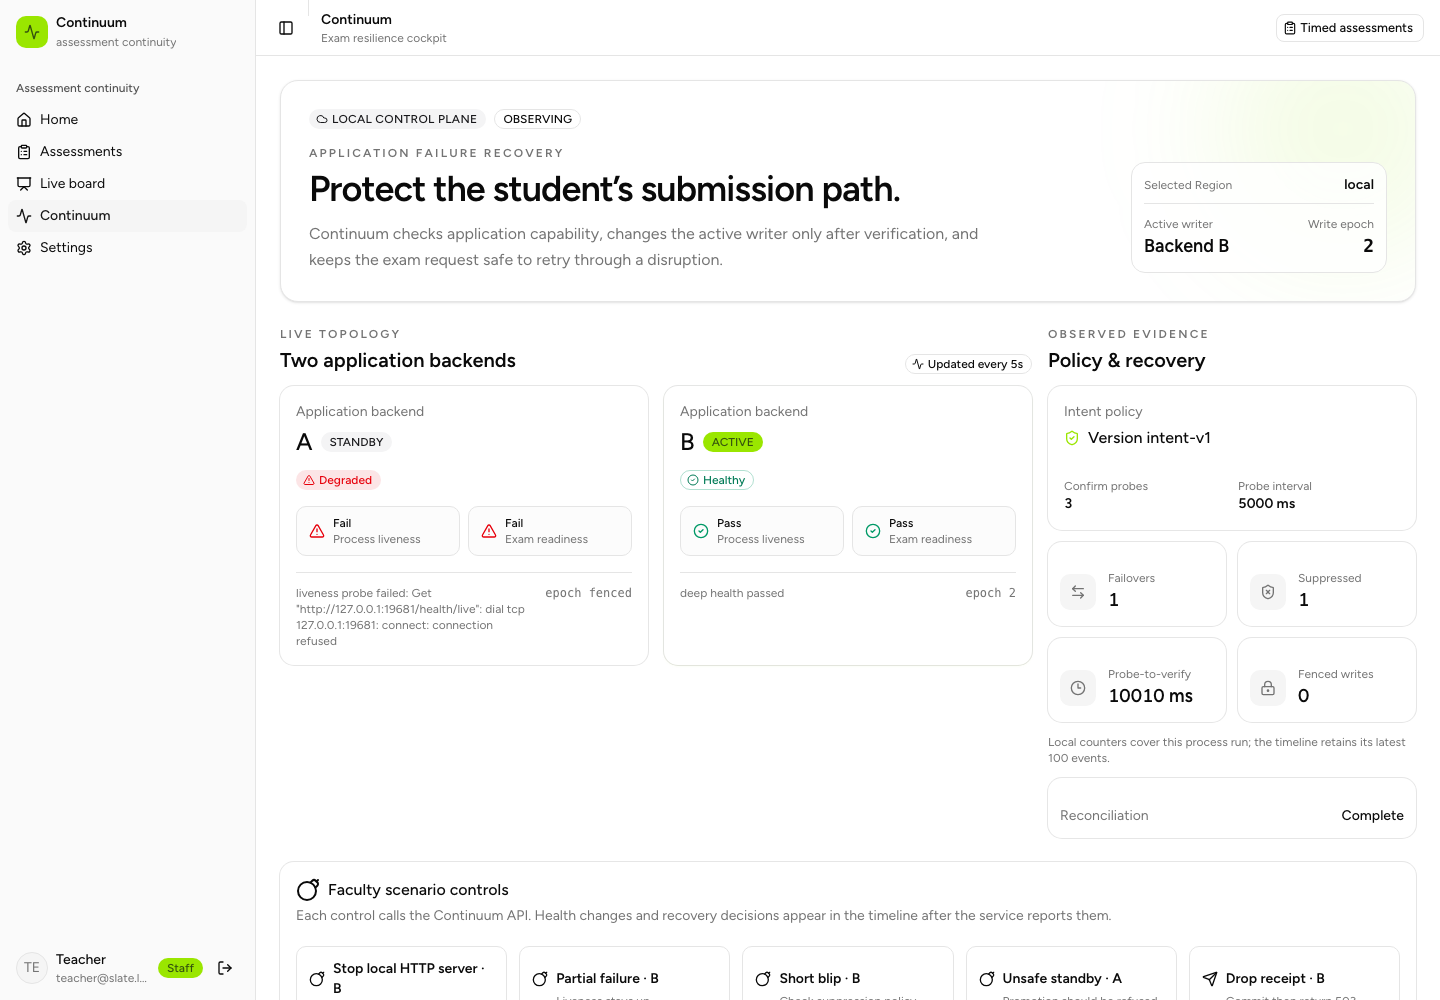
\includegraphics[width=\textwidth,trim=270bp 155bp 15bp 75bp,clip]{screenshots/recovery-local-promoted.png}
\caption[Local recovery to backend B at epoch 2]{Local recovery after stopping A's HTTP server: B is healthy and active at epoch 2; reconciliation is complete.}\label{fig:local-promoted}
\end{figure}

\begin{figure}[htbp]\centering
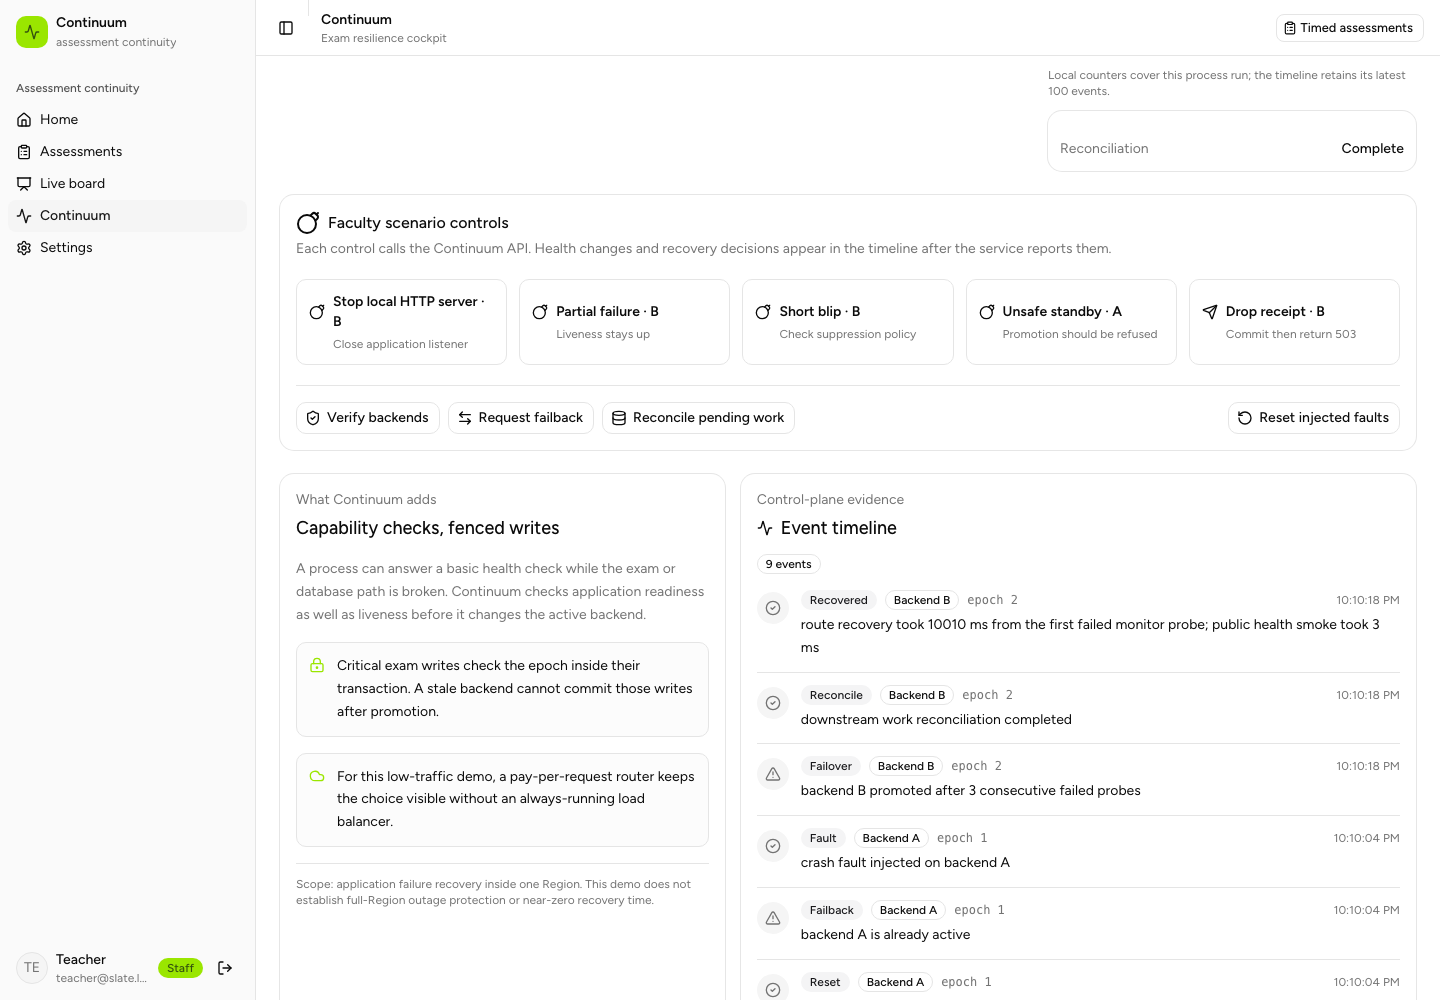
\includegraphics[width=112mm,trim=750bp 85bp 20bp 475bp,clip]{screenshots/recovery-event-timeline.png}
\caption[Local recovery event history]{Event history records the injected fault, promotion, public verification, and reconciliation. The list is ordered for operational viewing.}\label{fig:event-history}
\end{figure}

\FloatBarrier
\section{AWS Experiment Design}
The cloud rehearsal used two EC2 application instances in separate Sydney Availability Zones, a shared regional DynamoDB table, and the deployed routing and recovery services. A was initially active at epoch 1. Before the principal run, a 7.5-second transient fault recovered during confirmation, and an unsafe-standby case made both backends unready. Both suppressed promotion and retained epoch 1~\cite{cloud-run}.

The principal sequence combined a committed submission with an unavailable response:
\begin{enumerate}
\item Submit a fixed synthetic answer snapshot with a persistent request identifier. Commit succeeds, but injected response loss returns HTTP 503.
\item Request an actual stop of the active EC2 instance. Allow the scheduled monitor and workflow to determine the recovery action.
\item Observe B at epoch 2, verify public deep health, and inspect reconciliation.
\item Replay the unchanged request, then alter its payload under the same identifier and inspect the resulting conflict.
\item Independently count submission-related records and repeat reconciliation.
\end{enumerate}
This resolves one ambiguous committed outcome through a backend failure. It does not measure cohort throughput or continued writes during loss of DynamoDB.

\section{Recovery Timeline and Writer Authority}
Figure~\ref{fig:cloud-timeline} aligns events to the start of the instance-stop action. The workflow-start event appears at 41.940 seconds; promotion at 45.287 seconds, public verification at 45.470 seconds, and reconciliation at 47.970 seconds. External polling observed recovery at 50.472 seconds. These timestamps establish the sequence without identifying every internal scheduling or network delay.

\begin{figure}[htbp]\centering
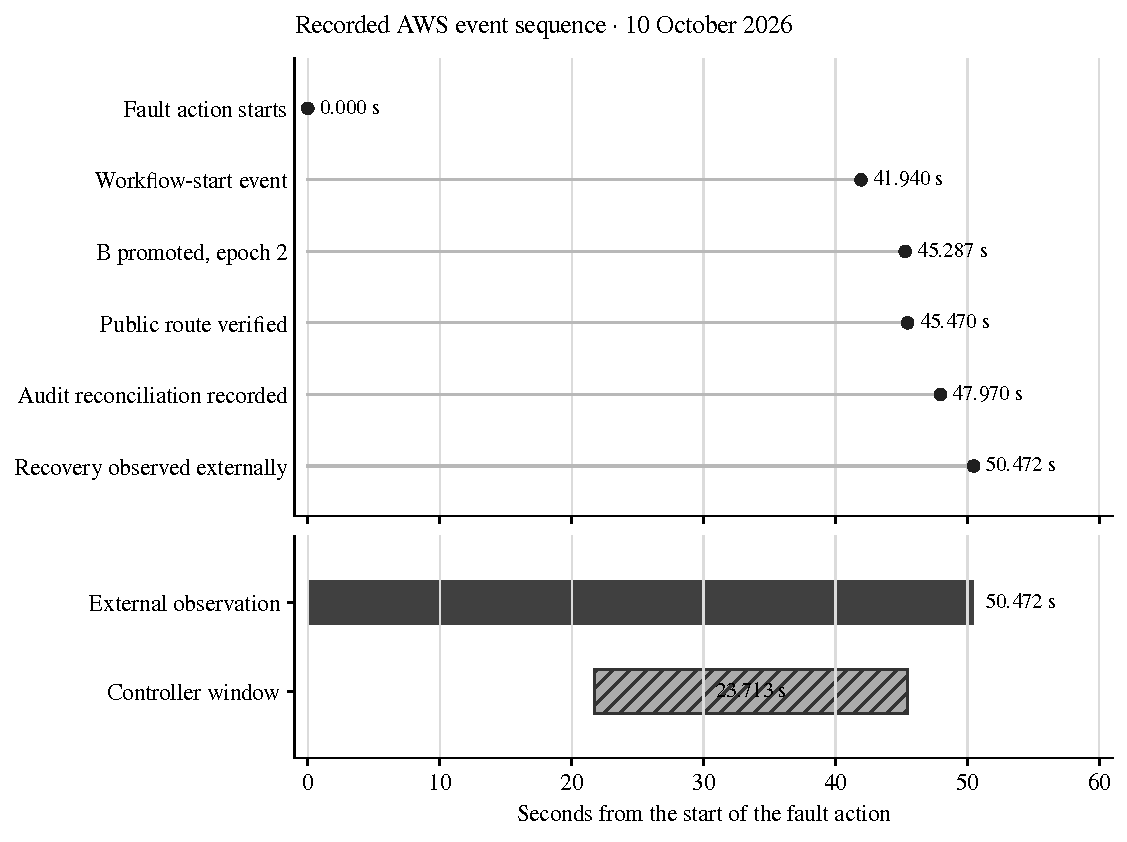
\includegraphics[width=\textwidth]{figures/cloud-timeline.pdf}
\caption[Recorded AWS event timeline and timing windows]{Recorded AWS event sequence and timing windows. The controller window's left endpoint is derived from the verification timestamp minus its recorded 23.713-second duration.}\label{fig:cloud-timeline}
\end{figure}

The external and controller intervals use different boundaries:
\begin{align}
T_{\mathrm{external}} &= t_{\mathrm{external\ observation}}-t_{\mathrm{fault\ action}}=50.472\,\mathrm{s},\\
T_{\mathrm{controller}} &= t_{\mathrm{public\ smoke}}-t_{\mathrm{check\ cycle\ start}}=23.713\,\mathrm{s}.
\end{align}
The controller interval begins before the workflow-start event because it includes monitoring and confirmation. Subtracting the durations does not isolate a single scheduling overhead: the endpoints differ, and external observation also includes polling and reconciliation. The preserved workflow result supplies the controller duration~\cite{cloud-records}.

\begin{figure}[htbp]\centering
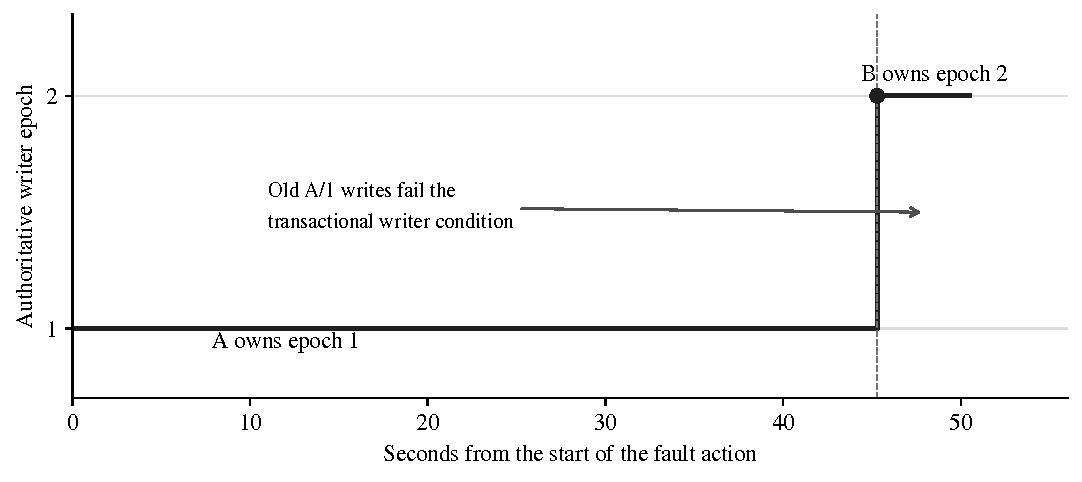
\includegraphics[width=\textwidth]{figures/writer-epoch.pdf}
\caption[Authoritative writer epoch transition]{Writer state reconstructed from the initial record and promotion event. Authority changes once from A/1 to B/2; restarting A does not grant it a newer epoch.}\label{fig:epoch-results}
\end{figure}

Figure~\ref{fig:epoch-results} represents authority, not merely process availability. An old in-flight transaction either commits before the promotion condition wins or fails the writer condition after it. Routing convergence alone would leave a period in which old A could still mutate shared data. The transactional fence closes that gap for protected writes.

\begin{figure}[htbp]\centering
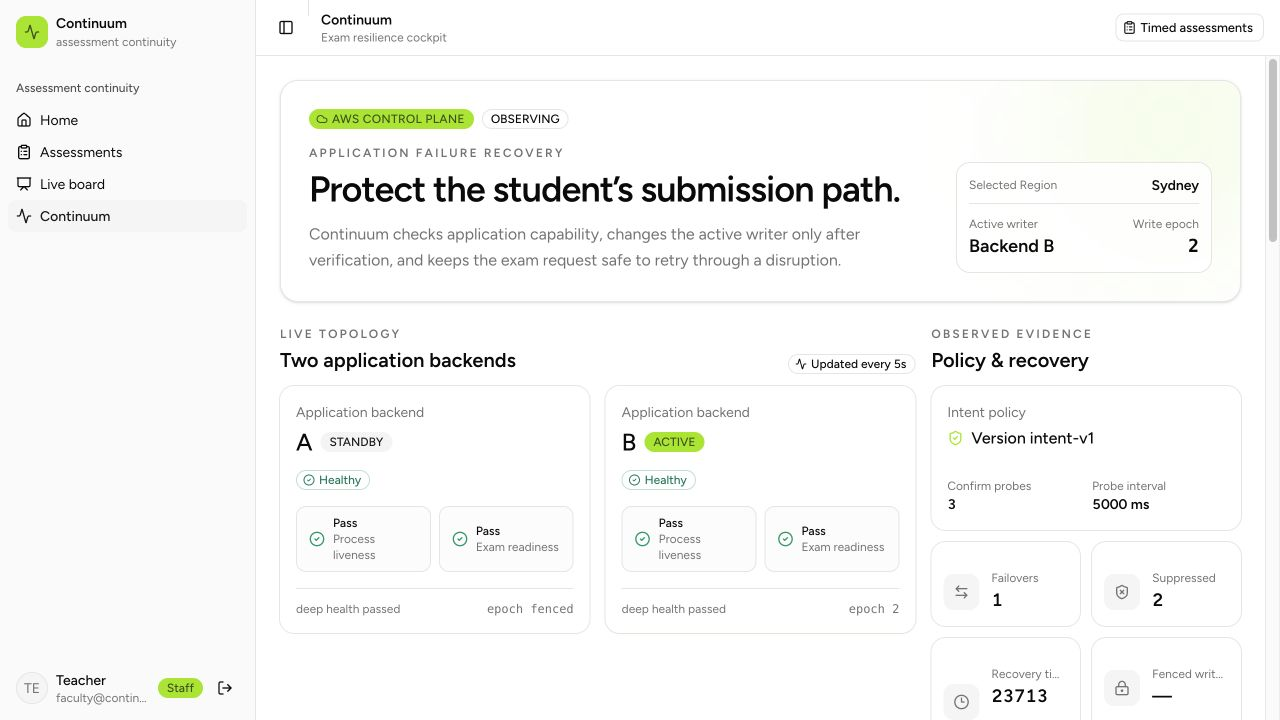
\includegraphics[width=\textwidth,trim=265bp 0bp 15bp 55bp,clip]{screenshots/cloud-recovery.png}
\caption[Recorded AWS recovery cockpit]{Preserved AWS cockpit from the cloud rehearsal, showing B active at epoch 2. This capture is separate from the new local demonstrations.}\label{fig:cloud-cockpit}
\end{figure}

\FloatBarrier
\section{Resolving the Lost Response}
The commit timestamp precedes the fault action by 1.609 seconds. Although the original request returned HTTP 503 after response loss, the exact retry returned a duplicate receipt with the original commit time. Here, duplicate means that the existing result was recovered, not that another submission was accepted.

\begin{table}[H]\centering\small
\caption{Recorded submission and replay comparison}\label{tab:receipt-comparison}
\begin{tabularx}{\textwidth}{@{}L{43mm}Y@{}}\toprule
\textbf{Field or operation} & \textbf{Recorded outcome}\\\midrule
Persistent request identifier & \texttt{cloud-6fbb0f1bc6fd4a86bdab2e9c17f33d23}\\
Original response after commit & HTTP 503 (deliberate response-loss injection)\\
Original commit timestamp & \texttt{1791652428408} milliseconds since the Unix epoch\\
Exact replay & \texttt{duplicate}; identical identifier and commit timestamp\\
Receipt scope and result & Attempt 1, version 1, score 2 of 5\\
Same identifier, changed answers & HTTP 409 conflict\\
Independent record inspection & One canonical submission, one receipt, one processed journal entry, one audit summary\\\bottomrule
\end{tabularx}\end{table}

The unchanged identifier and commit time answer the learner's question: the original submission exists despite the failed response. The changed-payload conflict establishes that the identifier cannot silently acquire another answer snapshot. Neither result follows merely from promoting a healthy standby.

\section{Reconciliation: Correctness and Work Performed}
The automatic recovery execution succeeded with one processed entry and zero conflicts. A repeated execution succeeded with zero new processed entries and zero conflicts. Independent inspection found one audit summary for the request~\cite{cloud-records}. Together, these support one logical downstream outcome for this inspected submission.

\begin{figure}[htbp]\centering
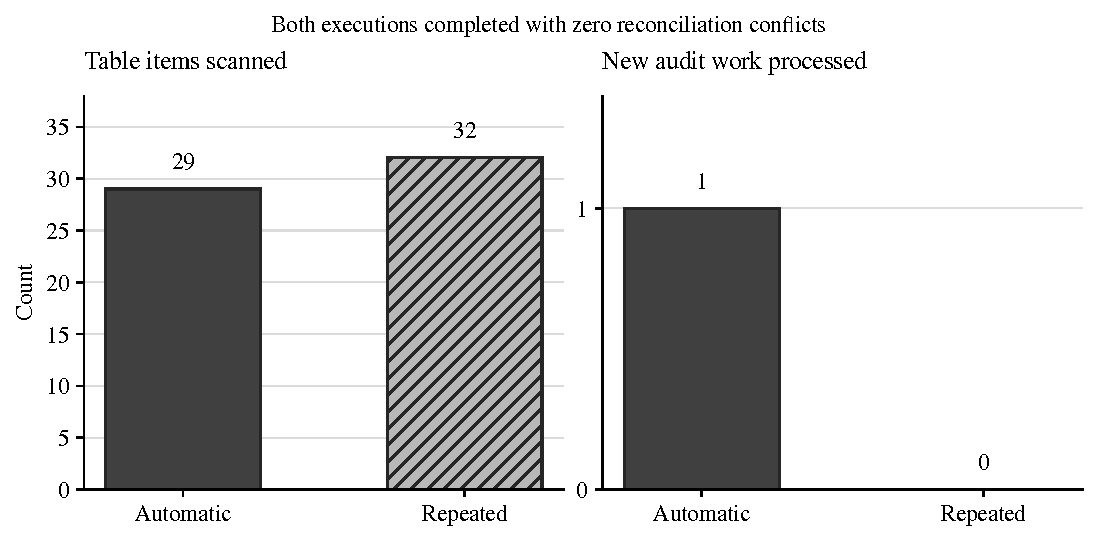
\includegraphics[width=\textwidth]{figures/reconciliation-work.pdf}
\caption[Observed reconciliation scans and new audit work]{Observed reconciliation: 29 and 32 table items scanned, with one and zero new audit outcomes. Scan count does not mean pending-submission count.}\label{fig:reconcile-work}
\end{figure}

The repeat still scanned 32 items. Idempotency prevents repeated business effects but does not make discovery free. The reconciler scans a table using an outbox filter, so \texttt{ScannedCount} can grow with unrelated data. A pending-work index or dedicated stream is a scaling improvement; this experiment does not establish that repeated scans remain efficient at institutional scale.

\section{Stale-Writer Validation}
After A restarted, a synthetic registration sent directly to A with epoch 1 returned HTTP 503 and \texttt{WRITER\_FENCED}. A strongly consistent email-index lookup found no created record~\cite{cloud-stale}. This checks stale registration specifically. Exam-submission fencing is covered by transactional storage and API tests; a stale exam submission was not sent directly to AWS in this rehearsal.



\section{Interpretation and Validity}
The strongest result combines route recovery, unchanged submission identity, and one inspected logical audit result. Suppression cases matter equally: a useful controller sometimes preserves the route rather than promotes. The local screens make decisions visible, while the AWS records establish the bounded cloud outcome.

Four limits constrain generalisation. One cloud run cannot establish mean or percentile recovery time, a production RTO, or an SLA. The workload is synthetic rather than a concurrent examination cohort. Shared DynamoDB, control services, and the selected Region remain dependencies. Finally, current-source checks and later local captures are dated separately from the preserved deployment. No data loss was observed for the inspected committed request, but this is not an unconditional zero-RPO guarantee.

\chapter{Security, Operations, and Cost}
\section{Security Design}
The public browser interfaces use HTTPS through CloudFront and API Gateway. The API authenticates application users and applies role and classroom access checks. Passwords are hashed, and student sessions do not grant access to fault injection. The recovery cockpit requires a separate administrator control token.

Network policy restricts application ingress to the router/verifier security group on port 8000. The deployment does not open inbound SSH; Systems Manager supports instance management. Backend traffic within the VPC uses HTTP in the prototype, which makes the private network boundary significant. Additional service-to-service transport protection is a production hardening requirement.

Runtime service roles provide AWS credentials to EC2 and Lambda. Bootstrap configuration is stored in an encrypted Systems Manager parameter, and the application bundle is retrieved from a private S3 bucket. Private runtime files, deployment outputs, and Terraform state must be protected because they can contain operational secrets.
\section{Separation of Service Permissions}
The application role can access the table for permitted application operations, including conditional checks on the active record. Explicit policy restrictions prevent it from writing the control and audit namespaces. The control function manages the active writer and instance operations, while the reconciler owns its bounded audit-processing responsibility.

The monitor is configured without the fault-control token. The workflow role invokes the functions needed for the recovery sequence. This distribution limits the authority of a component that only needs to observe or forward requests. The model concerns service permissions; human team-member access remains managed through the AWS project experience.
\section{Threat and Failure Considerations}

\begin{table}[H]\centering\small
\caption{Selected risks and implemented controls}\label{tab:risks}
\begin{tabularx}{\textwidth}{@{}L{41mm}Y@{}}\toprule
\textbf{Risk or failure} & \textbf{Control and remaining boundary}\\\midrule
Unauthorised fault action & Separate administrator token; credential protection remains essential\\
Forged or obsolete writer context & Private ingress plus database-enforced backend/epoch condition\\
Concurrent recovery actions & Incident lease, expected-state conditions, retry-safe promotion\\
Changed answers under one request ID & Scope and payload binding with conflict rejection\\
Misleading healthy process & Deep readiness and healthy-standby confirmation\\
Interrupted audit processing & Atomic outbox and conditional reconciliation\\
Private data in operational artifacts & Private state/output files; synthetic demonstration data\\
Shared regional dependency failure & Suppress unsafe promotion; outside the demonstrated recovery scope\\\bottomrule
\end{tabularx}\end{table}

The prototype is not presented as an institutional examination service ready for unrestricted use. Formal privacy review, retention policy, broader abuse controls, external security testing, backup/restore exercises, and operational ownership would be needed before using real examination data at scale.
\section{Operational Lifecycle}
Development and most rehearsals can use local mode. Cloud resources are enabled for bounded demonstration windows. The supported lifecycle is deploy, resume, verify both backends, perform the controlled scenario, capture the outcome, and pause the stack.

Before a cloud deployment, the selected Region is confirmed through AWS Settings, under View all projects, Overview, Additional Info, Region. The supported Terraform configuration validates Sydney and rejects another regional value. The project plan and current spend status are checked through AWS Settings and the plan API before resources are started. The recorded rehearsal used the Free plan; this historical fact does not establish a later credit balance.

Pause stops the EC2 instances and disables the monitoring schedule. Existing executions can finish, and retained disks, data, logs, or objects can continue to consume credits. Destruction is a separate action that removes persistent data as well as compute, so required synthetic results must first be retained deliberately.
\section{Monitoring Delay and Activity Models}
Monitoring frequency creates a direct trade-off between nominal detection delay and recurring work. The implemented scheduled monitor runs once per minute. Three confirmation probes have two five-second gaps, so even a fault discovered immediately requires a nominal ten seconds of confirmation spacing. Figure~\ref{fig:monitor-delay} explores one-, two-, and five-minute schedules; only the one-minute rate is the current deployment.

Let $S$ be the schedule period in seconds, $\phi\in[0,1]$ the fault's position within a schedule cycle, $p=3$ the number of probes, and $\delta=5$ seconds their spacing. An idealised model is
\begin{equation}
D_{\mathrm{nominal}}(S,\phi)=S(1-\phi)+(p-1)\delta.
\end{equation}
This excludes probe duration, schedule jitter, invocation latency, and subsequent workflow work. It is a planning model rather than a prediction or a bound on actual recovery. With uniformly distributed fault phase, its expected value is $S/2+10$: 40, 70, and 160 seconds for the three schedules.

\begin{figure}[htbp]\centering
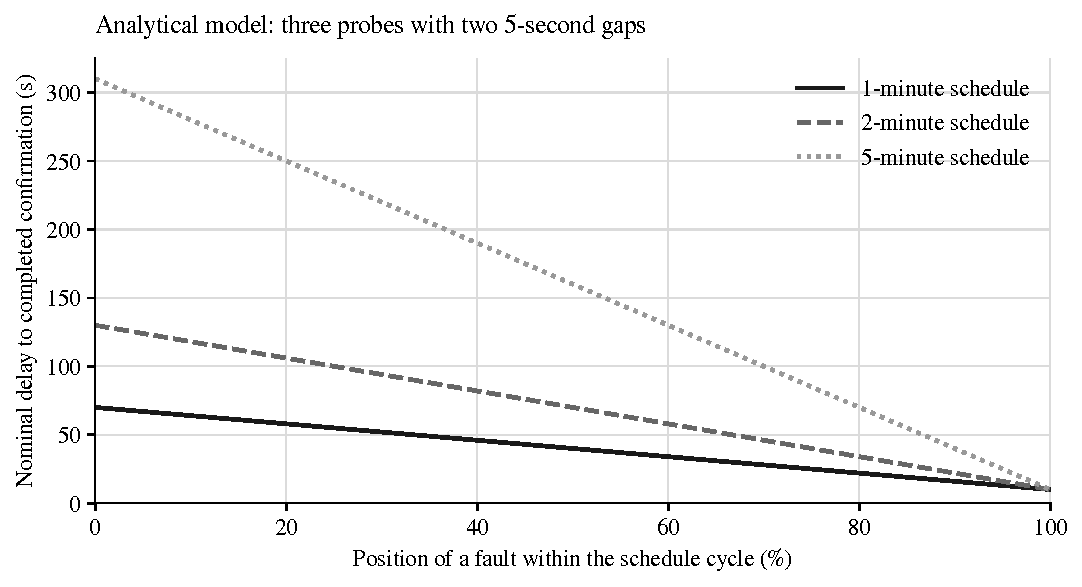
\includegraphics[width=\textwidth]{figures/monitor-phase-model.pdf}
\caption[Analytical monitoring and confirmation delay]{Analytical confirmation-delay scenarios, not measured performance. Faults just after a scheduled check wait almost a full cycle before confirmation can begin.}\label{fig:monitor-delay}
\end{figure}

For $h$ hours with monitoring enabled, the nominal scheduled activity is
\begin{equation}
N_{\mathrm{scheduled}}=\frac{3600h}{S}.
\end{equation}
At the implemented one-minute rate, a two-hour rehearsal produces 120 nominal monitor triggers and continuous daily operation produces 1,440. These counts exclude retries, manual invocations, and recovery workflow calls. They cannot be multiplied by a single unit price to obtain the entire cloud bill.

\begin{figure}[htbp]\centering
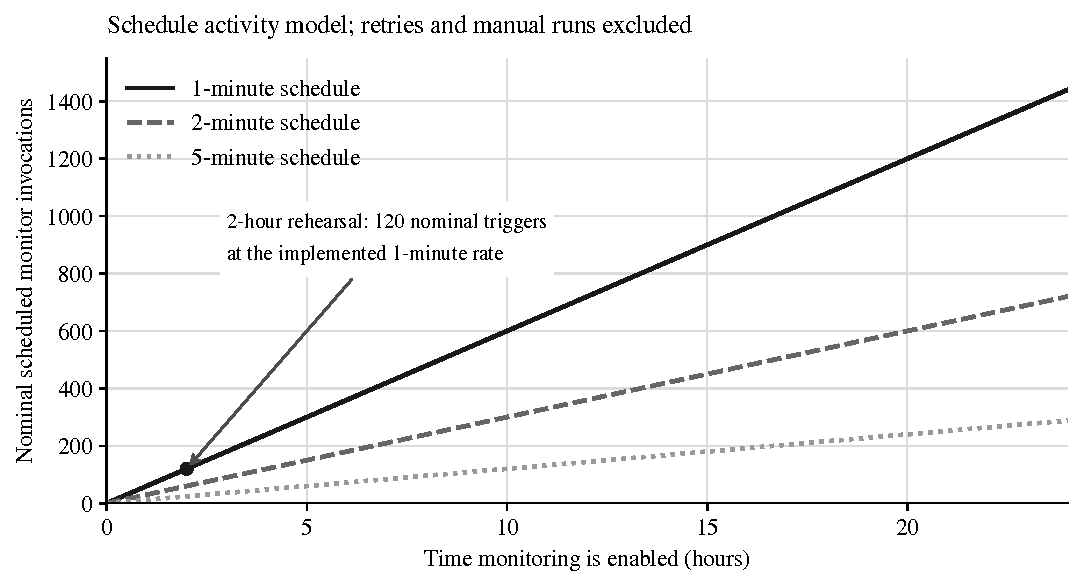
\includegraphics[width=\textwidth]{figures/monitor-activity-model.pdf}
\caption[Analytical scheduled monitoring activity]{Analytical monitoring activity against enabled hours. A slower schedule reduces recurring calls while increasing the phase-dependent wait shown in Figure~\ref{fig:monitor-delay}.}\label{fig:monitor-activity}
\end{figure}

The appropriate policy depends on the acceptable interruption and the cost of a false promotion. For this small demonstration, three probes suppress a short-lived fault and avoid reacting to a single failed request. Lower latency would require changing and validating the detection path, not simply claiming that public health recovery is instantaneous. Repeated trials with randomised fault phase should precede any production RTO claim.

\FloatBarrier
\section{Cost Model}
The major cost drivers are the two EC2 instances, their public IPv4 addresses while assigned, retained EBS volumes, DynamoDB operations and storage, Lambda invocations, API Gateway requests, workflow transitions, S3 objects, CloudFront delivery, and logs. Gateway VPC endpoints for S3 and DynamoDB have no additional endpoint charge~\cite{aws-endpoints}. The design avoids fixed NAT gateway and load-balancer resources.

A planning model separates active runtime from retained storage:
\begin{equation}
C_{\mathrm{period}}=2h(P_{\mathrm{EC2}}+P_{\mathrm{IPv4}})+C_{\mathrm{EBS}}+C_{\mathrm{requests}}+C_{\mathrm{storage}}+C_{\mathrm{delivery/logs}},
\end{equation}
where $h$ is the number of hours that both application instances are running. Rates depend on the selected Region and current pricing. This expression identifies cost drivers; it is not a fixed quotation or a guarantee that credits cover the deployment. Current EC2, VPC, and EBS rates should be checked for the actual rehearsal period~\cite{aws-ec2-price,aws-vpc-price,aws-ebs-price}.

The HTTP API stage is configured for a rate of three requests per second and burst capacity of six. No reserved Lambda concurrency is allocated. These values bound the demonstration and must not be treated as a capacity plan for a large cohort. Pause/resume, limited log retention, local rehearsal, and deterministic builds support efficient use of the available resources.
\section{Alignment with Cloud Architecture Principles}
The AWS Well-Architected Framework describes six pillars~\cite{aws-wellarchitected}. Table~\ref{tab:pillars} maps the implementation to those themes without claiming a formal framework review.

\begin{table}[H]\centering\small
\caption{Relationship to the Well-Architected pillars}\label{tab:pillars}
\begin{tabularx}{\textwidth}{@{}L{38mm}Y@{}}\toprule
\textbf{Pillar} & \textbf{Relevant project decision}\\\midrule
Operational excellence & Observable events, documented runbook, reproducible local checks\\
Security & Restricted ingress, service roles, separate operational token\\
Reliability & Standby verification, atomic fencing, receipt replay, outbox recovery\\
Performance efficiency & Bounded functions, timeouts, and explicit small-demo traffic limits\\
Cost optimisation & Local-first rehearsal, pause controls, absence of fixed NAT/load-balancer resources\\
Sustainability & Stop idle compute and retain only necessary demonstration artifacts\\\bottomrule
\end{tabularx}\end{table}


\chapter{Limitations, Future Work, and Conclusion}
\section{Current Limitations}
\subsection{Shared Data and Control Dependencies}
Both application instances depend on the same regional DynamoDB service. The router, API Gateway, Lambda, and workflow services are also part of the operating boundary. A complete Region outage or shared database failure cannot be repaired simply by changing the active application instance. No cross-Region replication or recovery path is part of the supported project.
\subsection{Timing and Capacity}
The monitoring schedule, confirmation probes, service invocation overhead, and client polling affect recovery time. The recorded values come from a single rehearsal and do not establish a production latency distribution. The API traffic limits and small instances are suitable for the bounded demonstration, while high-concurrency assessment traffic remains unvalidated.

A backend failure does not automatically extend a student's allowed time. The deadline calculation uses a persisted start time and mutable assessment duration, so administrator policy changes can affect an active attempt. Deadline validation also precedes the final storage call. A production assessment service should snapshot the effective policy and define whether acceptance is measured at request arrival, validation, or database commit. Exact receipt replay resolves an earlier commit; it does not authorise a new late answer.
\subsection{Deployment and Feature Coverage}
Local mode uses shared memory in one process and loses local state when the whole launcher restarts. It cannot demonstrate infrastructure isolation. Cloud mode uses separate instances and persistent regional storage, but the observed instance-stop experiment is not a complete Availability Zone outage test.

The broader product includes classroom collaboration and boards. The cloud recovery stack exposes the bounded HTTP assessment path and does not demonstrate WebSocket/board failover. Screenshots can also show a different frontend revision from a recorded cloud experiment; the request and data records are the authority for the specific measured replay outcome.
\Needspace{6\baselineskip}
\section{Future Work}
Useful extensions should preserve the existing submission and writer contracts:
\begin{itemize}
\item Measure repeated recovery trials across realistic traffic levels and report distributions with clearly defined timing boundaries.
\item Add production observability, alerting, tracing, and a documented response process for shared-service failures.
\item Exercise backup and restore, set explicit retention rules, and validate data handling before using real examination records.
\item Freeze effective attempt policy and test delayed writes across the deadline boundary, including concurrent changes to duration and availability.
\item Strengthen service-to-service transport protection and subject authentication, authorisation, and abuse controls to independent security testing.
\item Evaluate a production routing and capacity design while retaining transaction-level writer safety and durable request identity.
\item Define and test a separate recovery contract for collaborative boards and WebSockets if those features enter the cloud assessment scope.
\end{itemize}
\section{Conclusion}
Continuum demonstrates an application-centred approach to cloud recovery for timed assessments. It connects infrastructure failover with the correctness of the operation a student needs to complete. Readiness confirmation governs when recovery is justified, an incident lease serialises the decision, a monotonically increasing epoch assigns writer authority, and a database condition applies that authority at commit time.

Durable request receipts address the uncertainty created by a response lost after a successful commit. The transactional outbox permits pending audit work to complete without duplicating the logical outcome. Persisted attempt identity and start time provide continuity across backend changes under unchanged assessment metadata.

The Sydney rehearsal combined an actual EC2 stop, promotion, public verification, exact receipt replay, and independent record inspection. Backend tests complement these observations. Within the stated dependency boundary, Continuum demonstrates recovery of both an accessible service and a verifiable submission outcome.

\begingroup\fontsize{10}{11.5}\selectfont\setstretch{1.0}\setlength{\parskip}{0pt}
\begin{thebibliography}{99}
\fontsize{10}{11.5}\selectfont\setlength{\parskip}{0pt}\setlength{\itemsep}{4pt}
\addcontentsline{toc}{chapter}{References}
\bibitem{aws-transactions} Amazon Web Services, ``Amazon DynamoDB Transactions: How it works,'' \emph{Amazon DynamoDB Developer Guide}. \url{https://docs.aws.amazon.com/amazondynamodb/latest/developerguide/transaction-apis.html}. Accessed 23 October 2026.
\bibitem{aws-workflows} Amazon Web Services, ``Choosing workflow type in Step Functions,'' \emph{AWS Step Functions Developer Guide}. \url{https://docs.aws.amazon.com/step-functions/latest/dg/choosing-workflow-type.html}. Accessed 23 October 2026.
\bibitem{aws-endpoints} Amazon Web Services, ``Gateway endpoints,'' \emph{Amazon Virtual Private Cloud User Guide}. \url{https://docs.aws.amazon.com/vpc/latest/privatelink/gateway-endpoints.html}. Accessed 23 October 2026.
\bibitem{aws-lambda-vpc} Amazon Web Services, ``Enable internet access for VPC-connected Lambda functions,'' \emph{AWS Lambda Developer Guide}. \url{https://docs.aws.amazon.com/lambda/latest/dg/configuration-vpc-internet.html}. Accessed 23 October 2026.
\bibitem{aws-wellarchitected} Amazon Web Services, ``The pillars of the framework,'' \emph{AWS Well-Architected Framework}. \url{https://docs.aws.amazon.com/wellarchitected/latest/framework/the-pillars-of-the-framework.html}. Accessed 23 October 2026.
\bibitem{aws-ec2-price} Amazon Web Services, ``EC2 On-Demand Instance Pricing.'' \url{https://aws.amazon.com/ec2/pricing/on-demand/}. Accessed 23 October 2026.
\bibitem{aws-vpc-price} Amazon Web Services, ``Amazon VPC Pricing.'' \url{https://aws.amazon.com/vpc/pricing/}. Accessed 23 October 2026.
\bibitem{aws-ebs-price} Amazon Web Services, ``Amazon EBS Pricing.'' \url{https://aws.amazon.com/ebs/pricing/}. Accessed 23 October 2026.
\bibitem{project-source} Continuum source repository, current implementation: \path{internal/continuum}, \path{internal/clusterstate}, \path{internal/exams}, \path{internal/store}, \path{internal/httpapi}, \path{infra/demo}, and \path{statemachine/demo-failover.asl.json}. Source inspected 23 October 2026.
\bibitem{project-review} Continuum project documentation, \emph{Implementation and review evidence}, \path{docs/implementation-review.md}; \emph{Demonstration runbook}, \path{docs/demo-runbook.md}; and \emph{Product quality-of-life features}, \path{docs/qol-features.md}.
\bibitem{cloud-run} Continuum, recorded AWS rehearsal, 10 October 2026. Repository artifact: \path{docs/evidence/cloud-rehearsal.json}.
\bibitem{cloud-records} Continuum, independent AWS record and workflow inspection, 10 October 2026. Repository artifact: \path{docs/evidence/cloud-records.json}.
\bibitem{cloud-stale} Continuum, live stale-writer registration check, 10 October 2026. Repository artifact: \path{docs/evidence/cloud-stale-writer.json}.
\bibitem{local-capture} Continuum, local application capture, 23 October 2026. Synthetic BCSE355L classroom and assessment; original screens in \path{docs/report/screenshots/}, captured fault state and events in \path{docs/report/data/local-capture-summary.json}. Cloud graph measurements and analytical model parameters are included in \path{docs/report/data/}.
\bibitem{vit-logo} Vellore Institute of Technology, official VIT logo asset. \url{https://vit.ac.in/wp-content/uploads/2023/06/blue_logo-copy-scaled.webp}. Used on the cover page; accessed 23 October 2026.
\end{thebibliography}
\endgroup

\appendix\chapter{Reproducibility Guide}
\section{Local Execution}
The local launcher starts the frontend, public router, A/B HTTP servers, and shared memory store. Separate browser sessions distinguish the teacher/operator and learner. Credentials are read privately from the ignored runtime file.
\begin{lstlisting}
cd web
bun install --frozen-lockfile
cd ..
make demo-local
\end{lstlisting}
The default frontend address is \texttt{http://localhost:3000}; the cockpit is at \texttt{/ops}. Local mode labels its shared-process topology. A full launcher restart resets its in-memory data.
\section{Backend Verification Commands}
The six package suites in Table~\ref{tab:verification} were rerun using:
\begin{lstlisting}
go test -p 2 -race -timeout 5m \
  ./internal/continuum ./internal/store \
  ./cmd/demo-reconciler

go test -p 2 -race -timeout 5m \
  ./integration ./internal/httpapi ./internal/exams
\end{lstlisting}
The repository also supplies broader Go, frontend, build, Terraform, and browser checks. Their scope should be selected according to the part of the system changed.
\section{Controlled Recovery Demonstration}
\begin{enumerate}
\item Verify that both backends are ready, record the active backend and epoch, and start a fresh synthetic learner attempt.
\item Stop the active local HTTP server or, in an enabled AWS rehearsal, the active EC2 instance. Observe confirmation, promotion, and public verification.
\item Keep assessment policy unchanged and confirm that the learner's existing attempt start time continues to govern timing. Submit within the configured rules and retain the receipt.
\item Using a fresh suitable attempt, inject a post-commit response loss and retry the same request and answer snapshot. Compare its request ID and commit time.
\item Repeat reconciliation and inspect the canonical submission, receipt, processed outbox, and audit result. An unchanged logical outcome is required.
\item Restore a healthy baseline, exercise the brief-fault and unsafe-standby cases, and verify that inappropriate switches are suppressed.
\end{enumerate}
\section{Evidence and Operating Boundaries}
The preserved cloud artifacts are the rehearsal JSON, independent record/workflow inspection, and stale-registration check~\cite{cloud-run,cloud-records,cloud-stale}. Their results apply to the recorded synthetic scenarios. Assessment screenshots illustrate interface states and are not substitutes for request comparisons or database inspection.

Cloud execution requires a verified project plan, selected Region, current spend status, and healthy instances. Monitoring and compute should be paused after a bounded rehearsal. Resource destruction is separate from pause because it removes retained data.
\section{Rebuilding the Report and Graphs}
The LaTeX source package contains all included screenshots, vector diagrams, chart PDFs, whitelisted measurements, and chart-generation code. It compiles without a running application or an AWS connection:
\begin{lstlisting}
mkdir -p build
tectonic --keep-logs --outdir build main.tex
\end{lstlisting}
The charts are already included as vector PDFs. To regenerate them, install Python's Matplotlib and NumPy packages, then run:
\begin{lstlisting}
python figures/build_figures.py
\end{lstlisting}
The script reads \path{data/cloud-measurements.json}, exports the aligned event CSV, and writes five PDF/PNG chart pairs. Recorded measurements and analytical assumptions occupy separate data files. Screenshot crops in LaTeX change framing only; they do not alter the interface state or numerical results.

\end{document}
